% TEX root = ../main.tex
Si comincia ora l'introduzione alla Logica Proposizionale, 
partendo tuttavia da un concetto espresso senza formalizzarlo immediatamente: 
\begin{defi}[Enunciato]
Con il termine \textbf{enunciato} si intende una frase o un'espressione per la 
quale sia sensato chiedersi se sia vera o se sia falsa in ogni data 
circostanza, ossia ha un \textbf{valore di verità} relativo ad una 
certa circostanza. 
\end{defi}
``Piove'' è un enunciato, così come ``prendo l'ombrello'' 
e ``se piove prendo l'ombrello''. Sapremmo già dire che quest'ultimo ha 
qualcosa di diverso dai primi: quest'ultimo infatti è un \textbf{enunciato 
composto}, mentre i primi sono \textbf{enunciati atomici}. Ci sono frasi 
che non sono enunciati e possiamo anche limitarci all'italiano per trovarne 
alcuni: ``Paolo corre?'' e ``Piove?'' non sono enunciati. Oltre al linguaggio naturale 
vi sono anche altre frasi che non sono enunciati, per esempio ``2''. 

\section{Introduzione alla Logica Proposizionle}
\subsection{Senso, denotazione e connotazione di un enunciato}
Il senso filosofico di questi concetti verrà tralasciato e verranno infatti 
trattati in una maniera poco profonda, soprattutto per capire la distinzione
tra denotazione e connotazione. Ecco alcune espressioni del linguaggio 
dell'aritmetica: 
\begin{itemize}
  \setlength\itemsep{0pt}
  \item $4$
  \item $2^2$
  \item il predecessore di $5$ 
  \item $3+1$
\end{itemize}
Nessuno di questi è un enunciato, ma non è necessario che lo siano. 
Sappiamo dire cosa significhino, in quanto matematicamente sono sempre 
modi per esprimere \textit{il numero naturale quattro}. Questo esempio inquadra 
a livello intuitivo cosa sia la \textbf{denotazione} (il numero naturale 
quattro) e la \textbf{connotazione} (quattro diversi modi per ottenere quattro). 
Anche a livello intuitivo stiamo dicendo una cosa interessante, in quanto 
questo implica che dobbiamo essere molto precisi riguardo cosa dovrebbe
essere la \textit{denotazione} di qualcosa. 
Un'espressione ha, quindi, una denotazione che è qualcosa di diverso dalla 
sua connotazione. In un modo astratto, una espressione $E$ è un \textit{nome}
di qualcosa, come per esempio $4$, $2^2$, il predecessore di $5$ e $3+1$, 
il quale si riferisce in modo univoco a qualche entità. L'\textit{entità} alla 
quale si riferisce l'espressione è 
essa stessa la denotazione. La connotazione, in questo senso, è quanto 
l'espressione effettivamente esprime, ossia tutto il resto dell'informazione 
contenuta nell'espressione stessa. 

La logica studia la denotazione degli enunciati (chiamati anche \textit{sentences}) e 
non le connotazioni in quanto esse sono troppo difficili da gestire a livello 
iniziale. Le denotazioni godono infatti dell'importante proprietà dell'\textbf{invarianza 
per sostituzione}, ossia se ad un'espressione si cambiano delle parti 
sostituendole con parti denotazionalmente uguali, la denotazione globale 
non cambia, mentre la connotazione può potenzialmente cambiare totalmente, 
come dimostrano le quattro frasi iniziali.

\subsubsection{Denotazione di un Enunciato}
Si può definire ora, più formalmente, cosa sia la \textbf{denotazione} di 
un enunciato. Si prenda, per esempio, l'enunciato
$$
4 = \text{pred}(5)
$$
e si applichi una sostituzione con espressioni denotazionalmente equivalenti: 
$$
4 = 4
$$
Il principio d'invarianza dice che questi due enunciati sono \textbf{denotazionalmente}
equivalenti, benché l'ultimo enunciato non contiene nessuna informazione 
ulteriore rispetto alla denotazione stessa (circa). La denotazione 
di un enunciato è, quindi, il loro valore di verità, ossia il fatto che sono 
una forma connotazionale di una costante \texttt{vero} o \texttt{falso}. 
Quindi, l'oggetto della Logica Proposizionale sono le \textbf{proposizioni}, 
ossia il contenuto denotazionale degli enunciati, che può essere 
\texttt{vero} o \texttt{falso}. 

\subsection{Enunciati e Connettivi}
Alcuni enunciati semplici come ``Piove'' o ``Paolo corre'' sono definiti 
\textbf{atomici} in quanto la loro denotazione è solamente un valore di 
verità. Altri enunciati, definiti \textbf{composti}, sono enunciati che si possono
``smontare'', come ``Piove e c'è vento'', che è chiaramente composto 
dagli enunciati atomici ``Piove'' e ``c'è vento''. Il connettivo ``e'' è 
ciò che li unisce, come potrebbe accadere anche per ``o'', ``non'' 
e ``se...allora''. 

In una maniera più formale, gli enunciati semplici 
devono solamente rappresentare il fatto che denotano un valore di verità e 
saranno quindi rappresentati da \textbf{simboli} appartenente all'insieme infinito
$L$ chiamato \textbf{linguaggio proposizionale}. I simboli 
$p, q, r, p_1, \cdot \in L$ sono chiamati \textbf{lettere proposizionali}. 
Oltre alla sintassi, formalmente il valore semantico (quindi denotazionale) di ogni 
lettera proposizionale è un valore di verità. 

Gli enunciati composti sono formalizzabili con una simbologia che rispetta 
i simboli per gli enunciati atomici: $p \land q$, $p \lor q$, $\neg p$ e 
$p \rightarrow q$ sono enunciati composti. I simboli $\land, \lor, \neg$ 
e $\rightarrow$ sono chiamati \textbf{connettivi}. Il valore denotazionale 
di ogni enunciato composto dipenderà dai 
valori denotazionali degli enunciati atomici e dal valore semantico dei connettivi 
che lo compongono. 

\section{Sintassi della Logica Proposizionale}
Si può ora formalizzare la struttura sintattica degli enunciati: 
l'insieme $F_{L}$ degli enunciati costruibili 
sul linguaggio $L$ rispettando la \textbf{sintassi 
degli enunciati} è definito come segue: 
\begin{itemize}
  \setlength\itemsep{0pt}
 \item $F_L$ è il più piccolo insieme tale che 
    \begin{itemize}
      \item per ogni $p \in L$ si ha $p \in F_L$
      \item se $A,B \in F_L$ allora anche $(A\land B) \in F_L$, $(A\lor B) \in F_L$, 
        $(A \rightarrow B) \in F_L$ e $(\neg A) \in F_L$, dove $A$ e $B$ possono 
        essere a loro volta enunciati complessi. 
      \end{itemize}
  \item $F_L$ è l'intersezione di tutti gli insiemi $X$ tali che 
    \begin{itemize}
      \item $L \subseteq X$
      \item se $A,B \in X$ allora $(A\land B)$, $(A\lor B)$, $(\neg A)$ e 
        $(A \rightarrow B)$ sono contenuti in $X$. 
    \end{itemize}
  \item (induttiva) $F_L$ è l'insieme che rispetta le condizioni seguenti: 
    \begin{itemize}
      \item $L \subseteq F_L$: se $p \in L$, allora $p \in F_L$
      \item Se $A,B \in F_L$, allora $(A\land B)$, $(A\lor B)$, $(\neg A)$ e 
        $(A \rightarrow B)$ sono contenuti in $F_L$
      \item Nient'altro appartiene a $F_L$.
    \end{itemize}
\end{itemize}

\paragraph{Esercizio}
Scrivere qualcosa che non sia un enunciato utilizzando solamente la sintassi della 
logica proposizionale. Un esempio è $p q \neg$. Un altro è $\rightarrow q$.

\subsection{L-Costruzioni}
Per stabilire se una stringa $w \in (\{\land, \lor, \neg, \rightarrow\}
\cup L)*$\footnote{L'utilizzo dell'operatore $*$ è paragonabile all'operatore 
  Stella di Kleene nella Teoria dei Linguaggi e denota l'insieme di tutte le
  stringhe di lunghezza finita componibili utilizzando le lettere 
  dell'alfabeto indicato, in questo caso i connettivi e le lettere 
proposizionali.}
è anche $w \in F_L$ si utilizza una \textbf{L-costruzione} o 
\textbf{certificato}, ossia una sequenza finita di formule $w_1, w_2, \cdots, w_n$ tale che 
per ogni $i = 1,\cdots, n$ si ha $w_i \in L$, ossia 
$w$ è una lettera proposizionale, oppure esiste $j < i$ tale 
che $w_i = \neg w_k$, ossia $w_i$ è la forma negata 
di una formula più semplice che appare prima nell'elenco di 
formule; oppure esistono $k,j < i$ tali per cui 
$w_i = w_k \land w_j$ o $w_i = w_k \lor w_j$ o $w_i = w_k \rightarrow w_j$.
Sia, per esempio $w = ((p\land q)\rightarrow w)$. Per dimostrare che 
è $w \in F_L$ si possono introdurre come L-costruzione 
$w_1 = p, w_2 = q, w_3 = (p\land q), w_4 = r$ e infine $w_5 = (p \land q) \rightarrow r$; 
questa L-costruzione \textit{certifica} che $w \in F_L$.
In termini computazionali, si può controllare velocemente che quanto fatto 
sopra sia una costruzione corretta e che pertanto $w \in F_L$. Si noti, inoltre, 
che questa L-costruzione non è unica. 
I certificati portano con sé una proprietà importante riguardo le formule, 
ossia 
\begin{pro}[di unica leggibilità dei Certificati]
Se $w \in F_L$, allora vale uno e uno solo dei seguenti casi: o $w \in L$, 
o esiste $v$ tale che $w = \neg v$, o esistono $v_1, v_2$ tali che 
$w = (v_1 \land v_2)$, 
$(v_1 \lor v_2)$ o $(v_1 \rightarrow v_2)$, dove i $v_i$ sono determinati 
univocamente. 
\end{pro}
Questa proprietà garantisce l'esistenza di una sorta di operazione 
inversa della costruzione di certificati: mentre quest'ultimo ``monta'' 
una formula, questa proprietà garantisce il fatto che sia possibile 
``smontarla'' in un unico modo.
Questa proprietà non è condivisa tra tutti i linguaggi formali: per 
esempio nelle grammatiche una stringa $w = ciao$ può essere composta da $v_1 = \epsilon$ 
e $v_2 = ciao$ eccetera. 
Spesso, il concetto di leggibilità può essere espresso anche tramite il concetto 
di \textbf{albero di parsing} di una formula, che è unico e mostra come 
essa sia costruita. 

\subsection{Osservazioni e convenzioni riguardo alla sintassi}
Esistono ulteriori connettivi (o derivati) oltre a quelli utilizzati fino ad ora, 
ossia $\land$, $\lor$, $\neg$ e $\rightarrow$: 
uno di questi è $\bot$, che è un connettivo di arità zero che denota il falso; un 
altro è $\top$, che è un connettivo zerario che denota il
sempre vero e chiaramente $\bot = \neg \top$. Altro connettivo è $\iff$, 
definito come $(A \rightarrow B) \land (B \rightarrow A)$.

Una seconda osservazione riguarda l'uso delle parentesi: per come abbiamo definito 
le formule, l'oggetto $p \land q \notin F_L$ in quando mancano le parentesi. 
In formule complesse, le parentesi possono aggiungere complicatezza e portare l'errore: 
useremo il buonsenso per ``dimenticarci'' delle parentesi laddove non ci sia 
pericolo di confusione. Tuttavia non bisogna farsi trasportare troppo, in quanto 
esistono delle parentesi necessarie, come per esempio $(p \land q ) \lor r)$ 
oppure $p \land (q \lor r)$. 

\section{Semantica della Logica Proposizionale Classica}
Per dare una definizione di semantica si utilizzano due princìpi guda: il 
\textbf{principio di bivalenza} e il \textbf{principio di verofunzionalità}. 
\begin{pri}[Bivalenza]
Un enunciato, in ogni circostanza, è o vero o falso.
\end{pri}
Il principio di bivalenza ha come conseguenza il principio del terzo escluso. 
\begin{pri}[Verofunzionalità, composizionalità o estensibilità]
Il valore di verità di un enunciato composto dipende solo dal valore di verità 
degli enunciati che lo compongono e dal significato del connettivo che li unisce. 
\end{pri}
Dato il principio di verosimiglianza, per dare la semantica ad un connettivo come $\land$
si deve dire qual è, sotto ogni circostanza, il valore di verità di $A \land B$, 
il quale può essere \texttt{vero} o \texttt{falso} e può dipendere solo dal valore 
di verità di $A$ e $B$ e dal significato fissato per $\land$. 
Una \textbf{circostanza} è un assegnamento che definisce lo stato vero 
o falso di una lettera proposizionale (o di una formula), definita come 
una funzione $\mathfrak{v}$:
$$
\mathfrak{v} : L \rightarrow \{0,1\}
$$
e quindi $\mathfrak{v}(A \land B) \in \{0,1\}$ dipende solo da $\mathfrak{v}(A)$, 
$\mathfrak{v}(B)$ e dal significato fissato per $\land$, definito come 
$$
I_{\land}: \{0,1\}^2 : \{0,1\}
$$
E si ha, quindi
$$
\mathfrak{v}(A \land B ) = I_{\land} (\mathfrak{v}(A), \mathfrak{v}(B))
$$

Si supponga per un attimo che invece di Logica si stia studiando Probabilità, 
tentando di formalizzarla come stiamo formalizzando ora la Logica Proposizionale. 
Siamo in una circostanza in cui un certo evento ha probabilità
$v(A) = \frac{1}{2}$ e un altro evento ha probabilità $v(B) = \frac{1}{2}$. 
La probabilità $v(A \rightarrow A) = 1$ rappresenta l'evento certo. 
Qual è la probabilità $v(A \rightarrow B)$? Se fossimo in una situazione verofunzionale, 
questa probabilità dovrebbe essere $1$, in quanto se $v(\frac{1}{2} \rightarrow \frac{1}{2}) = 1$, 
allora uguale anche per $v(A \rightarrow B) = 1$. Per concretezza, si immagini 
$A = $ domani piove e $B = $ a Pasqua nevica.  In conclusione, la 
verofunzionalità è una caratteristica stringente della Logica Proposizionale 
da non dare affatto per scontata. 

Siamo finalmente pronti per dare una definizione formale della 
\textbf{semantica} della Logica Proposizionale: 
\begin{defi}[Semantica della Logica Proposizionale]
Un assegnamento (o valutazione) è un'arbitraria funzione 
$$
\mathfrak{v} : L \rightarrow \{0,1\}
$$ 
che formalizza la nozione intuitiva di circostanza (o \textit{mondo possibile}). 
La \textbf{semantica dei connettivi} è espressa tramite delle funzioni:
$$
I_{\land} : \{0,1\}^2 : \{0,1\}
$$
che identificano una \textit{tabella di verità}. Una volta definita quest'ultima, 
si può definire la \textbf{semantica degli enunciati}: essa è l'\textbf{estensione canonica}
$$
\widetilde{\mathfrak{v}}: F_L \rightarrow \{0,1\}
$$
ossia l'estensione di $\mathfrak{v}$ a tutte le formule, definita in questo modo: 
\begin{itemize}
  \item $\widetilde{\mathfrak{v}}(p) = \mathfrak{v}(p)$ se $p \in L$
  \item $\widetilde{\mathfrak{v}}(A \land B) = I_{\land}(\widetilde{\mathfrak{v}}(A), \widetilde{\mathfrak{v}}(B))$ se $p \in F_L$
  \item $\widetilde{\mathfrak{v}}(A \lor B) = I_{\lor}(\widetilde{\mathfrak{v}}(A), \widetilde{\mathfrak{v}}(B))$se $p \in F_L$
  \item $\widetilde{\mathfrak{v}}(A \rightarrow B) = I_{\rightarrow}(\widetilde{\mathfrak{v}}(A), \widetilde{\mathfrak{v}}(B))$ se $p \in F_L$
  \item $\widetilde{\mathfrak{v}}(\neg A) = I_{\neg}(\widetilde{\mathfrak{v}}(A))$ se $p \in F_L$
\end{itemize}
\end{defi}

\noindent
in modo induttivo, come è accaduto anche per $F_L$.
Vi sono inoltre delle forme algebriche per esprimere i valori di verità dei connettivi, 
per esempio 
$$
\widetilde{\mathfrak{v}}(A \rightarrow B) = min\{1-\widetilde{\mathfrak{v}}(A), \widetilde{\mathfrak{v}}(B)\}
$$
\subsection{Nozioni Semantiche Fondamentali}

\begin{defi}[Tautologia]
Una formula $F \in F_L$ è una tautologia se e solo se 
$$
\mathfrak{v}(F) = 1 \forall \mathfrak{v} : L \rightarrow \{0,1\}
$$
\end{defi}
\begin{defi}[Formula Soddisfacibile]
Una formula $F \in F_L$ è soddisfacibile se e solo se 
$$
\exists \mathfrak{v}:L \rightarrow \{0,1\} : \mathfrak{v}(F) = 1
$$
\end{defi}
\begin{defi}[Contraddizione]
Una formula $F \in F_L$ è una contraddizione (o insoddisfacibile, refutabile) se e solo 
se 
$$
\mathfrak{v}(F) = 0 \forall \mathfrak{v}: L \rightarrow \{0,1\}
$$
\end{defi}
C'è un fatto molto semplice che lega tra di loro questi concetti: 
\begin{teon}
$F \in F_L$ è una tautologia se e solo se $\neg F$ è insoddisfacibile. 
\end{teon}
\begin{proof}
  $F$ è tautologica se e solo se $\widetilde{\mathfrak{v}}(F) = 1$ per 
  ogni $\mathfrak{v}: L \in \{0,1\}$, ossia se e solo se $\widetilde{\mathfrak{v}}(\neg F) 
  = 0$ per ogni $\mathfrak{v}: L \in \{0,1\}$, ossia $\neg F$ è insoddisfacibile. 
\end{proof}

\subsubsection{Principio d'Induzione su $F_L$}
Benché non sia una sfaccettatura prettamente semantica, in quanto verrà 
(anzi, è già stato) utilizzato abbondantemente, è importante formalizzare 
il  \textbf{principio d'induzione}. Sia 
$P$ una proprietà delle formule; si ha che 
$P$ vale per ogni formula $F \in F_L$ se e solo se: 
\begin{enumerate}
  \item \textbf{(base):} $P$ vale per ogni $p \in L$
  \item \textbf{(passo induttivo)}: se $P$ vale per $A,B  \in F_L$, allora 
    vale anche per $\neg A$, $A \rightarrow B$, $A \lor B$ e $A \land B$. 
\end{enumerate}

Si può dimostrare induttivamente una proprietà anche grazie 
alla definizione  induttiva di $F_L$. Sia $I = \{ F \in F_L : P \text{ vale per } F\}$
Vogliamo mostrare $I = F_L$, ossia che $I$ è esattamente l'insieme di tutte le formule; 
questo si dimostra mostrando che $I \subseteq F_L$ e che $F_L \subseteq I$. 
\`E ovvio, per definizione, che $I \subseteq F_L$ in quanto è definito 
come un sottoinseme di formule. Per dimostrare il contrario, is dimostra che 
$I$ soddisfa il primo punto della definizione induttiva di $F_L$, ossia contiene 
tutte le lettere proposizionali (dalla base induttiva) e anche il secondo, in  quanto 
se $A,B \in I$ allora anche $(\neg A)$, $(A \rightarrow B)$, $(A \land B)$ e 
$(A \lor B)$. Grazie al terzo punto della definizione di $F_L$, si può inoltre affermare 
che in quanto non sono contenute altre formule in $I$ (per definizione) $I = F_L$.
Come esempio, si dimostra induttivamente il seguente lemma: 
\begin{lem}[Verità di una Formula]
Sia $F \in F_L$ e siano $\mathfrak{v}, \mathfrak{v}' : L \rightarrow \{0,1\}$. 
Se $\mathfrak{v}(p) = \mathfrak{v}'(p) \forall p \in L \in F$, 
allora $\widetilde{\mathfrak{v}}(F) = \widetilde{\mathfrak{v}}'(F)$.
\end{lem}
\begin{proof}
  \textit{Per induzione su } $F$. 
  \begin{itemize}
    \item \textbf{base:} Se $F = p \in L$ allora per ipotesi $\mathfrak{v}(p) = \mathfrak{v}'(p)$ e 
      anche $\widetilde{\mathfrak{v}}(p) = \widetilde{\mathfrak{v}}'(p)$.
    \item Se $F = \neg A$ allora per ipotesi induttiva 
      $\widetilde{\mathfrak{v}}(p) = \widetilde{\mathfrak{v}}'(p)$ e $\widetilde{\mathfrak{v}}(F) = 1 - 
      \widetilde{\mathfrak{v}}(A) = 1 - \widetilde{\mathfrak{v}}'(A) = \widetilde{\mathfrak{v}}'{F}$
    \item Se $F = (A \land B)$ per ipotesi induttiva $\widetilde{\mathfrak{v}}(A) = \widetilde{\mathfrak{v}}'(A)$ 
      e $\widetilde{\mathfrak{v}}(B) = \widetilde{\mathfrak{v}}'(B)$ e pertanto 
      $\widetilde{\mathfrak{v}}(F) = \min\{\widetilde{\mathfrak{v}}(A), \widetilde{\mathfrak{v}}(B)\} = 
      \min\{\widetilde{\mathfrak{v}}'(A), \widetilde{\mathfrak{v}}'(B)\} = \widetilde{\mathfrak{v}}'(F)$.
    \item uguale per gli altri connettivi.
  \end{itemize}
\end{proof}
Il lemma appena provato ci garantisce che se vogliamo calcolare $\widetilde{\mathfrak{v}}(F)$ 
ci basta calcolare la tabella di verità di $F$. A questo punto si può calcolare, 
per ogni assegnamento, se una formula è vera, soddisfacibile, tautologica o 
insoddisfacibile.

\paragraph{Esercizio}
Date $A, B \in F_L$ si esaminino le seguenti formule. 
La formula $A \land \neg A$ è insoddisfacibile in quanto 
\begin{table}[!h]
  \centering
  \begin{tabular}{|c|c|}
  \hline
  $A$ & $A \land \neg A$ \\
   0  &   0        \\ 
   1  &  0         \\
   \hline
 \end{tabular}
\end{table}

La formula $A \rightarrow \neg A$ è soddisfacibile ma non tautologica 
in quanto 
\begin{table}[!h]
  \centering
  \begin{tabular}{|c|c|}
    \hline 
    $A$ & $A \rightarrow \neg A$\\
     0 &   1 \\
     1 &  0 \\
     \hline
  \end{tabular}
\end{table}

Si noti come è stato detto che $A,B$ siano state definite come appartenenti 
all'insieme delle formule e non alle lettere ($L$), ``imbrogliando'', un poco, 
rispetto al lemma precedente. Tuttavia, $A$ e $B$ possono essere considerate 
come \textit{metavariabili} a prescindere dalla loro complessità. Non è invece 
possibile fare il contrario, ossia considerare lettere come delle formule: 
per esempio, non è possibile dire che una lettera sia una tautologia. 

\paragraph{Esercizio}
Verificare che le seguenti siano Tautologie per ogni $A,B \in F_L$:
\begin{enumerate}
  \item $A \rightarrow (B \rightarrow A)$ (Weakening, Prefixing)
  \item $(\neg A \rightarrow A) \rightarrow A$ (Consequentia Mirabilis)
  \item $(A \rightarrow B) \lor (B \rightarrow A)$ 
  \item $(A \rightarrow B) \rightarrow (\neg B \rightarrow \neg A)$ (Contronominale)
  \item $(A \land B) \rightarrow A$
  \item $A \lor \neg A$  (Tertium non datur)
  \item $\bot \rightarrow A$ (Ex Falsum Quodlibet Sequitur)
\end{enumerate}

\begin{defi}[Tautologia]
Se la formula $F$ è una tautologia, si indicherà 
$$
\models F
$$
\end{defi}


\subsection{Nozioni Semantiche Fondamentali per Insiemi di Formule}
Sia $\Gamma \subseteq F_L$ un insieme di formule. $\Gamma$ è detto 
\textbf{teoria} ed è un modello per un mondo in cui tutte le formule che 
gli appartengono sono vere. Si dice che $\Gamma$ è soddisfacibile 
se e solo se  $\exists \mathfrak{v}: L \rightarrow \{0,1\} : \forall \gamma \in \Gamma ~~ \mathfrak{v}(\gamma) = 1$
o, in notazione alternativa, $\mathfrak{v} \models \gamma$ e contestualmente 
si dice $\mathfrak{v} \models \Gamma$. Al contrario se e solo se 
$\forall \mathfrak{v}: L \rightarrow \{0,1\} ~~ \exists \gamma \in \Gamma : \mathfrak{v}(\gamma) = 0$, 
la teoria $\Gamma$ è insoddisfacibile e $\mathfrak{v} \nvDash \gamma$ e 
$\mathfrak{v} \nvDash \Gamma$. 

\begin{defi}[Conseguenza Logica]
Sia $\Gamma \subseteq F_L$ e $A \in F_L$. La formula $A$ è una 
\textbf{conseguenza logica} di $\Gamma$ se e solo se 
$$
\forall \mathfrak{v}: L \rightarrow \{0,1\} : \mathfrak{v} \models\gamma \in \Gamma
$$ 
(quindi $\mathfrak{v} \models\Gamma$) e $\mathfrak{v} \models A$. 
Si denoterà questo fatto con la notazione $\Gamma \models A$.
\end{defi}

\paragraph{Esercizio} 
Esprimere il concetto di formula tautologica o tautologia ($\models A$)
attraverso il concetto di conseguenza logica. 
Quando si ammette una teoria, si restringe il campo dei possibili assegnamenti. 
Una formula è tautologica quanto è vera in ogni circostanza ed è verificata 
da ogni assegnamento. Sia $\Gamma$ definito in questo modo. $\Gamma \subseteq F_L$ 
un insieme composto solo da tautologie. Allora 
$\Gamma \models A$. Dato che è sempre meglio avere come teoria la più semplice 
possibile, si può definire $\Gamma = \emptyset$, concludendo $\emptyset \models A$. 

\noindent
Ogni tanto si può utilizzare la notazione $\Gamma \cup \{A\} \models B$, che 
a volte viene semplificato in $\Gamma,A \models B$. 

\subsubsection{Proprietà semantiche Fondamentali delle Teorie}

\begin{lem}[Conseguenza Logica di una Formula da una Teoria insoddisfacibile]
Sia $\Gamma \subseteq F_L$ una teoria e $A \in F_L$. Si 
ha che $F \models A$ se e solo se $\Gamma \cup \{\neg A \}$ è insoddisfacibile. 
\end{lem}

\begin{proof}
Dimostriamo che $\Gamma \models A$ se e solo se 
$\mathfrak{v} \models \gamma \forall \gamma \in \Gamma \rightarrow \mathfrak{v}\models A$, 
in altre parole per ogni assegnamento di verità tale che $\mathfrak{v} \models \Gamma$ 
si ha $\mathfrak{v}(A) = 1$.
Si può tradurre quanto scritto utilizzando la definizione di implicazione materiale, 
ossia 
\begin{align*}
  &\neg (\mathfrak{v} \models \gamma \forall \gamma \in \Gamma) \lor \mathfrak{v}\models A \\
  \iff &\neg (\mathfrak{v}(\gamma) = 1 \forall \gamma \in \Gamma) \lor \mathfrak{v}(A) = 1\\
  \iff & (\exists \gamma \in \Gamma : \mathfrak{v}(\gamma) = 0) \lor \mathfrak{v}(\neg A) = 0 \\
  \iff & \exists B \in \Gamma \cup \{\neg A\}: \mathfrak{v}(B) = 0  \\
  \iff & \Gamma \cup \{\neg A\} \text{ è insodd.}
\end{align*}
\end{proof}

\begin{lem}[Deduzione, semantico] Siano $P$, $Q$ due formule. Allora 
si dice che $P \models Q$ se e solo se $\models P \rightarrow Q$. 
\end{lem}
\begin{proof}
Assumiamo che $P \models Q$. Per definizione, 
$\forall \mathfrak{v}: L \rightarrow \{0,1\}:\mathfrak{v}(P) = 1 \rightarrow \mathfrak{v}(Q) = 1$. 
Assumendo, quindi, che ogni volta che $\mathfrak{v}(P) = 1$ si ha $\mathfrak{v}(Q) = 1$, 
si ha direttamente che $\models P\rightarrow Q$, in quanto sostanzialmente 
si rimuove la possibilità di avere $P$ vero e $Q$ falso.
\end{proof}

Il teorema generalizza il lemma alla seguente situazione. 
\begin{teo}[Deduzione,semantico]
Sia $\Gamma$ una teoria 
e $P$, $Q$ formule. Allora $\Gamma,P \models Q$ se e solo se
$\Gamma \models P \rightarrow Q$. 
\end{teo}
\begin{proof}
Si dimostra dicendo che $\Gamma, P \models Q$ se e solo se 
$\forall \mathfrak{v}: L \rightarrow \{0,1\}: \mathfrak{v}(\gamma) = 1 \forall \gamma \in \Gamma$ e 
$\mathfrak{v}(P) = 1$ si ha che $\mathfrak{v}(Q) = 1$. Questo avviene se e solo se 
$\forall \mathfrak{v}:L \rightarrow \{0,1\} : \mathfrak{v}(\gamma) = 1$ si ha $\mathfrak{v}(P \rightarrow Q) = 1$ 
e segue per definizione $\Gamma, P \models Q$. 
\end{proof}

\subsection{Teorema di Compattezza}
Il teorema di compattezza è un teorema fondamentale della logica e varrà 
anche per la logica del prim'ordine. Lo proviamo ora per la logica proposizionale. 
\`E in qualche modo, in forma astratta, un teorema di completezza. 

Prima di mostrare l'enunciato, si introduce il concetto. \`E stata data la 
nozione di teoria, $\Gamma \in F_L$: ci si chiede se serve, nella logica 
proposizionale, considerare teorie infinite (composte da un numero 
infinito di formule). A priori, sembrerebbe proprio di sì e si vedrà affrontando
la Logica del Prim'Ordine che una singola formula al Prim'Ordine contiene informazioni 
di un numero infinito di formule proposizionali; questo basta per giustificare il caso 
in cui $\Gamma$ sia una teoria infinita. Il punto è che non sembra possibile 
gestire la teoria infinita: qui torna utile il teorema di compattezza. 
 

Il teorema di compattezza permette di ridurre l'analisi della soddisfacibilità di 
una teoria eventualmente infinita all'esame della soddisfacibilità dei suoi 
sottoinsiemi finiti. Tuttavia, è ovvio che il numero di sottoinsiemi finiti 
sia infinito. 
\noindent

Si enuncia, ora, il teorema di compattezza.
\begin{teo}[Compattezza]
Un insieme $\Gamma \subset F_L$ è soddisfacibile se e solo se lo è ogni
$\Gamma' \subseteq \Gamma$, con $\Gamma'$ finito, con notazione: $\Gamma' \subseteq_{\omega} \Gamma$ (leggasi 
``$\Gamma '$ sottoinsieme finito di $\Gamma$'').
\end{teo}
La dimostrazione consiste nel 
provare che la parte destra implica la parte sinistra, ossia 
che se ogni $\Gamma ' \subseteq_{\omega} \Gamma$ è 
soddisfacibile allora lo è anche $\Gamma$, in quanto l'altro 
verso è ovvio dalla definizione di soddisfacibilità di una teoria, mentre
il fatto che sottoinsiemi di $\Gamma$ siano soddisfacibili non implica ovviamente 
che $\Gamma$ sia soddisfacibile. 

\subsubsection{Prova}
Definiamo $\Gamma$ \textit{finitamente soddisfacibile} se per ogni $\Gamma' \subseteq_{\omega} \Gamma$ 
si ha che $\Gamma'$ è soddisfacibile. Il succo della dimostrazione sarà la relazione tra 
finitamente soddisfacibile e soddisfacibile, ossia 
si proverà che $\Gamma$ finitamente soddisfacibile implica $\Gamma$ soddisfacibile. 
Fissato un elenco o successione $F_1, F_2, \cdots, F_k, \cdots$ senza 
ripetizioni di tutte le formule in $F_L$, si costruisce ora una successione 
infinita di insiemi di formule $D_0, D_1, \cdots, D_k, \cdots$ definita induttivamente
sull'indice $i$ di $D_i$. Sia 
$$
D_0 = \Gamma
$$ 
e 
$$
D_{n+1} = 
\begin{cases} 
  D_n \cup \{F_{n+1}\} & \text{se } D_n \cup \{F_{n+1}\} \text{ è finitamente soddisfacibile} \\
  D_n \cup \{\neg F_{n+1}\} & \text{altrimenti}
\end{cases}
$$
si definisce infinine $D = \cup_{i \in \mathbb{N}} D_i$. 

Si possono provare ora alcuni fatti riguardanti $D_i$ e $D$. In primis, 
ogni $D_n$ per ogni naturale $n$ è finitamente soddisfacibile. Questo si basa 
sull'induzione sull'indice $n$: $n = 0$ implica $D_0$ finitamente soddisfacibile 
dato che $D_0 = \Gamma$ che è finitamente soddisfacibile per ipotesi. Per $n \neq 0$, si suppone 
che questo fatto sia vero per $D_0, \cdots, D_n$ e si prova vero per $D_{n+1}$. 
Per mostrare $D_{n+1}$ finitamente soddisfacibile si procede per assurdo e si assume 
$D_{n+1}$ non finitamente soddisfacibile in modo di arrivare ad una contraddizione: 
non si sa che forma abbia $D_{n+1}$ e bisogna provare che entrambi i casi 
portano al fatto che non sia finitamente soddisfacibile. Se non sono finitamente 
soddisfacibili, allora esiste un insieme $D' \subseteq_{\omega} D_{n}\cup \{F_{n+1}\}$ 
tale che $D'$ è insoddisfacibile ed esiste $D''\subseteq_{\omega} D_{n} \cup \{\neg F_{n+1}\}$
tale che $D''$ è insoddisfacibile. Senza perdita di generalità, si può assumere che 
$F_{n+1} \in D'$ e $\neg F_{n+1} \in D''$; in altre parole $D' = E' \cup \{F_{n+1}\}$ 
e $D'' = E'' \cup \{\neg F_{n+1}$ e si può affermare che $E', E'' \subseteq D_{n}$ 
e $F_{n+1} \notin E'$, $\neg F_{n+1} \notin E''$.

Si noti che gli insiemi $E' \cup E'' \cup \{F_{n+1}\}$ e $E' \cup E'' \cup 
\{\neg F_{n+1}\}$ sono insoddisfacibili perché contengono $D'$ e $D''$ rispettivamente, 
ma $E' \cup \subseteq_{\omega} D_{n}$ e per ipotesi induttiva $D_n$ è 
finitamente soddisfacibile, ed è quindi $E' \cup E''$ soddisfacibile ed esiste 
un assegnamento $v$ tale che $\mathfrak{v} \models E' \cup E''$. Sappiamo che 
$\mathfrak{v}(F_{n+1})$ è uguale a $0$ o a $1$ e pertanto non è possibile che entrambi
$\{F_{n+1}\}$ e $\{\neg F_{n+1}\}$ siano falsi. 
Abbiamo raggiunto la contraddizione che conclude la prova per assurdo 
mostrando $D_{n+1}$ finitamente soddisfacibile. Questo chiude a sua volta la 
prova per induzione, mostrando che ogni $D_n$ per $n \in N$ è finitamente 
soddisfacibile. 
 
In secondo luogo, $D = \cup_{i \in \omega} D_i$ è a sua volta finitamente 
soddisfacibile. Questo non è necessariamente ovvio a partire dal fatto 
che $D$ sia l'unione di insiemi finitamente soddisfacibili.
Si consideri un sottoinsieme finito $D' \subseteq_{\omega} D$. Per dimostrare 
che $D'$ sia finitamente soddisfacibile, si può pensare di elencarne 
i membri $D' = \{F_{i_1}, F_{i_2},\cdots,F_{i_u}\}$. Sia $k = \max_{j=1}^{u} i_j$; 
allora, $D' \subseteq_{\omega} D_k$, ma per il primo fatto $D_k$ p 
finitamente soddisfacibile e si può concludere $D'$ finitamente soddisfacibile
e $D$ finitamente soddisfacibile.

Il terzo fatto da dimostrare è che per ogni formula o enunciato $F_t$ esattamente 
una tra $F_t$ e $\neg F_t$ appartiene a $D$. Anche questo non è necessariemente 
garantito, in quanto $F_{n+1}$ e $\neg F_{n+1}$ non hanno lo stesso indice, 
ossia $\neg F_{n+1}$ non ha indice ${n+1}$. La dimostrazione di questo fatto 
arriva col  ragionamento seguente: per costruzione della sequenza dei $D_i$ 
$F_t$ o $\neg F_t$ appartiene a $D_t$ e quindi, dato che ogni $D_t \subseteq D$ 
si ha $F_t \in D$ o $\neg F_t \in D$. Bisogna escludere che ci siano entrambe, 
e che quindi la congiunzione ``o'' diventi uno xor. Si ha che $\{F_t, \neg F_t\} \nsubseteq D$, 
perché altrimenti per il secondo fatto $D$ è finitamente soddisfacibile e si avrebbe 
che $\{F_t, \neg F_t\}$ è soddisfsacibile, ma è assurdo, dato che ovviamente 
non può essere soddisfacibile per la semantica della negazione. 

Infine, si definisce l'assegnamento $v_D : L \rightarrow \{0,1\}$:
per ogni $p \in L$ si ha $v_D(p) = 1 \iff p \in D$. Si noti che $v_D$ è ben 
definito in quanto necessarimente $p \in D$ o $p \notin D$. L'ultimo fatto 
afferma che $v_D \models D$, che significa che $\forall F \in D v_D(F) = 1$. 
Se questo fatto è vero, allora è vero che $v_D \models Gamma$ dato che $\Gamma \subseteq D$, 
dunque $\Gamma$ è soddisfacibile. Questo fatto si dimostra per induzione 
strutturale l'affermazione seguente: per ogni $F \in F_L$ $v_D(F) = 1$ se 
e solo se $F \in D$. Questo non è uguale alla definizione precedente, in quanto 
in principio è stato definito per le lettere proposizionali e non per la 
funzione estesa ($\tilde{v}_D$). Ci basterebbe provare che $F \in D$ 
implica $v_D(F) = 1$ ma per convenienza proviamo anche che $v_D(F) = 1$ implica 
$F \in D$. La base induttiva è che $F = p$ e $p \in L$, l'asserto da 
provare segue dalla definizione di $v_D$. Il passo induttivo si svolge esaminando 
i connettivi uno per volta. Se $F = \neg G$, allora 
$v_D(F) = 1 \iff v_D(G) = 0 \iff G \notin D \iff \neg G \in D \text{ dal fatto tre }\iff F \in D$. 

Se $F = (G \land H)$ allora $v_D(F) = 1 \iff v_D(G \land H) = 1 \iff v_D(G) = 1 \land v_D(H) = 1\iff G \in D \land G \in D$. Questo ultimo fatto è dimostrabile perché se $G, H \in D$ allora 
$G \land G \in D$, poiché altrimenti se $\neg(G \land H) \in D$ implicherebbe 
che $\{G, H, \neg \{G \land H\}\} \subseteq_{\omega} \in D$ finitamente 
soddisfacibile, assurdo; e se $G\land H \in D $ allora $G, H \in D$, poichè altrimenti 
$G \notin D$ o $H \notin D$. Questo implica che $\{G\land H, \neg G\}$ 
o $\{G\land H, \neg H\} \in D$ siano finitamente soddisfacibili, assurdo. 
 
Se $F = (G \lor H)$ allora $v_D(F) = v_D(G \lor H) \iff v_D(G) = 1 \lor v_D(H) = 1 \iff G \in D \o H \in D$
allora se $G \in D$ o $H \in D$ allora $G \lor H \in D$ poiché altrimenti 
se $G \lor H \notin D$ allora $\neg (G \lor H) \in D$ se $G \in D$ allora 
$\{G, \neg \{G \lor H \} \subseteq_{\omega} D$
o se $H \in D$ allora $\{H, \neg \{G \lor H\} \subseteq_{\omega} D$ finitamente 
soddisfacibili, assurdo; se $G \lor H \in D$ allora $G \in D$ o $H \in D$, 
poiché altrimenti se $G \notin D$ e $H \notin D$ allora $\neg G \in D $ e 
$\neg H \in D$ e $\{\neg G, \neg H, \{G \lor H \}\} \subseteq_{\omega} D$ 
finitamente soddisfacibile, impossibile. 

\subsubsection{Prova contronominale}
$\Gamma$ è insoddisfacibile se 
e solo se $\exists \Gamma' \subseteq_{\omega} \Gamma$ e $\Gamma'$ è 
insoddisfacibile. 
\paragraph{$\rightarrow$ contronominale} 
Se c'è $\Gamma' \subseteq_{\omega} \Gamma$ insoddisfacibile, allora $\Gamma$ 
è insoddisfacibile in quanto $\Gamma$ è più restrittivo di $\Gamma'$, ha 
meno assegnamenti di $\Gamma'$ che possono soddisfarlo. 

\paragraph{$\leftarrow$ contronominale}
Se $\Gamma$ è insoddisfacibile, allora esiste $\Gamma' \subseteq_{\omega} \Gamma$, 
$\Gamma'$ insoddisfacibile. 

\subsubsection{Osservazioni sul Teorema di Completezza}
L'idea di dimostrare la validità del teorema di compattezza partendo 
da una teoria composta da un insieme infinito di formule per creare una catena 
di insiemi 
$$
\Gamma = D_0 \subseteq D_1 \subseteq D_2 \cdots \subseteq D_k \cdots \subseteq D
$$
è curioso. Si può concludere inoltre che $D$ non può essere ulteriormente ampliato 
senza perderne la soddisfacibilità, in quanto se $F \notin D$ $\overline{D} = D \cup \{F\}$ 
non è soddisfacibile, in quanto $F \notin D$ implica $\neg F \in D$.
Questo vuol dire che $D$ è un \textbf{ampliamento massimale} di $\Gamma$. 

\begin{defi}[Insieme massimale soddisfacibile]
  Si definisce \textbf{insieme massimale soddisfacibile} 
  ogni sottoinsieme $E \subseteq F_L$ tale che 
$E$ è soddisfacibile e $\forall F \in F_L : F\notin E$ si ha che $E \cup \{F\}$ è 
non soddisfacibile. 
\end{defi}
$D$ è solo uno di tali insiemi ed è quello che è stato 
costruito a partire da $\Gamma$. $D$ è un ampliamento massimale di $\Gamma$ o 
\textit{un} ampliamento di $\Gamma$? 
Pragmaticamente, se si elencano le formule in modo differente si ottiene, in genere, 
un ampliamento differente.
A livello delle informazioni contenute, un insieme massimale soddisfacibile $D$ 
si comporta come un assegnamento. Per ogni assegnamento $\mathfrak{v} : L \rightarrow \{0,1\}$ 
si può creare $D_\mathfrak{v} = \{ F \in F_L : \mathfrak{v}(F) = 1\}$, un 
insieme massimale soddisfacibile. 
Il teorema di compattezza verrà usato per decidere i casi in cui $\Gamma \models A$. 
Infatti, per un lemma che abbiamo già dimostrato, $\Gamma \models A \iff \Gamma \cup \{\neg A \} $
è insoddisfacibile. Si supponga che $\Gamma$ sia una teoria finita, 
$\Gamma = \{B_1, \cdots, B_n\}$ e si vuole sapere se $\Gamma \models A$. 
Questo è vero se e solo se $B_1, \cdots, B_n \models A \iff \{B_1, \cdots,B_n,\neg A\}$ è 
insoddisfacibile, se e solo se $B_1 \land \cdots B_n \land \neg A$ è 
insoddisfacibile. Se, invece, $\Gamma$ è infinito viene finalmente in 
nostro aiuto il teorema di compattezza. 

\subsection{Equivalenza Semantica}
Sintatticamente, come enunciati, cioè come stringhe di simboli, le 
due formule 
$$
A \lor B
$$ 
e 
$$
B \lor A 
$$ 
sono due formule differenti, nonostante $A$ sia $A$ e $B$ 
sia $B$: sono \textit{scritte} in modo diverso. Il loro \textbf{significato}, 
tuttavia, è uguale e, pertanto, per ogni $\mathfrak{v} : L \rightarrow \{0,1\}$ si ha che 
$\mathfrak{v}(A \lor B) \equiv \mathfrak{v}(B \lor A)$. Quella appena 
definita è una \textbf{relazione}. 

\begin{defi}[Relazione]
  Una relazione $n$-aria $R$ su un insieme $S$ è 
un sottoinsieme dell'insieme di tutte le $n$-ple di tutti gli elementi di $S$, 
in altre parole $R \subseteq S^{n}$.
\end{defi}
Per esempio, una relazione binaria è 
una relazione $R$ su $S$ tale che $R \subseteq S^2$. 
\begin{defi}[Relazione di equivalenza]
Una 
\textbf{relazione d'equivalenza} è una relazione binaria $R$ su $S$, $R \subseteq S^2$ 
tale che 
\begin{itemize}
  \setlength\itemsep{0pt}
  \item $R$ è riflessiva: $\forall s \in S ~~(s,s) \in R$
  \item $R$ è simmetrica: $\forall s_1, s_2 \in S ~~ (s_1, s_2) \in R \rightarrow (s_2, s_1) \in R$
  \item $R$ è transitiva: $\forall s_1, s_2, s_3 \in S ~~ (s_1, s_2), (s_2, s_3) \in R \rightarrow (s_1, s_3) \in R$
\end{itemize}
\end{defi}

\subsubsection{Partizioni e classi di equivalenza}
Sia $R$ una relazione di equivalenza su $S$. Per ogni $s \in S$, la 
\textbf{classe di equivalenza} rispetto ad $R$ di $s \in S$ è definita 
$$
[s]_R = \{ t \in S : (s,t) \in R\}
$$
\`E importante osservare che se $(s,t) \in R$ allora $[s]_R = [t]_R$ e viceversa, 
ossia se $[s]_R = [t]_R$ allora $(s,t) \in R$.  Una \textbf{partizione} di 
un insieme $S$ è un insieme $\{B_1, \cdots, B_k, \cdots\}$ non necessariamente 
finito di sottoinsiemi di $S$ ($B_i \subseteq S$) tale che $B_i \cap B_j = \emptyset$ 
per ogni $i,j \in I$, dove $I$ è l'insieme di indici di $B$. Inoltre, 
$\cup_{i \in I} B_i = S$. Gli insiemi $B_i$ vengono chiamati \textit{blocchi}
della partizione. I due concetti, partizioni e relazioni di equivalenza, sono 
legati tra di loro: ogni relazione di equivalenza $R$ su $S$ determina una partizione 
$P_R$ di $S$ dove 
$$
P_R = \{[s]_R : s \in S\}
$$
ossia le classi di equivalenza definite da $R$. La relazione inversa è meno nota, 
ossia che ogni partizione $P$ di $S$ determina una relazione d'equivalenza $R_P$ 
su $S$, ossia 
$$ 
R_P := (s,t) \in R_p \implies \exists i : s,t \in B_i
$$
che è chiaramente riflessiva, simmetrica e transitiva. 

\subsubsection{Equivalenza Logica}
Verificare che la relazione seguente (equivalenza logica $\equiv$) è d'equivalenza: 
$$ 
\equiv \subseteq F_L^2
$$
$$
\forall A,B: (A,B) \in \equiv \forall \mathfrak{v}:L\rightarrow \{0,1\} \mathfrak{v}(A) = \mathfrak{v}(B)
$$
\begin{enumerate}
  \item $\equiv$ riflessiva: $A \equiv A$ infatti $\forall \mathfrak{v}:L \rightarrow \{0,1\} \mathfrak{v}(A) = \mathfrak{v}(A)$
  \item $\equiv$ simmetrica: per ogni $(A,B) \in F_L^2$ se $A \equiv B$ allora
    $B \equiv A$, ossia se per ogni assegnamento $\mathfrak{v}:L \rightarrow \{0,1\}$ si 
    ha che $\mathfrak{v}(A) = \mathfrak{v}(B)$ allora per ogni $v$ si ha $\mathfrak{v}(B) = \mathfrak{v}(A)$. 
  \item $\equiv$ transitiva: per ogni $(A,B,C) \in F_L^3$ se $A \equiv B$ e 
    $B \equiv C$ allora $A \equiv C$ (dalla transitività della funzione 
    $=$ stessa). 
\end{enumerate}

$\equiv$ partiziona $F_L$, infatti 
$$
P_{\equiv} = F_L/\equiv =  \{ [A]_{\equiv} : A \in F_L\}
$$
\noindent 
\subsubsection{Sostituzione di lettera proposizionale con Formula}
Arricchiremo l'insieme delle classi di equivalenza delle formule, rispetto 
all'equivalenza logica, con delle operazioni che equipaggeranno tale insieme 
di una struttura algebrica.
Siano $A, B \in F_L$ una formula e sia $p \in L$ una lettera proposizionale. 
Si definisce la formula che si ottiene sostituendo nella formula $A$ ogni 
occorrenza della formula $B$ con la lettera proposizionale $p$
$$
A[B/p]
$$
induttivamente, con l'idea che per esempio data $(p \land \neg q)$ si ha 
$[(t \rightarrow q)/p] = (t\rightarrow q) \land \neg q$. 
\newline
\textbf{base:} $A = q, q \in L$  allora 
\begin{align*}
  q[B/q] := 
  \begin{cases}
    B & p = q \\
    q & p \neq q 
  \end{cases}
\end{align*}
\newline
\textbf{passo:}  
$(\neg A)[B/p] := \neg(A[B/p])$, 
$(A_1 \land A_2)[B/p] := (A_1[B/p]) \land (A_2[B/p])$, 
$(A_1 \lor A_2)[B/p] := (A_1[B/p]) \lor (A_2[B/p])$, 
$(A_1 \implies A_2)[B/p] := (A_1[B/p] \implies A_2[B/p])$. 

\begin{lem}[di sostituzione]
Sia $\mathfrak{v}: L \rightarrow \{0,1\}$ e siamo $S,T \in F_L$. 
Se $\mathfrak{v}(S) = \mathfrak{v}(T)$,  allora per ogni $A \in F_L$ e ogni $p \in L$
$$
\mathfrak{v}(A[S/p]) = \mathfrak{v}(A[T/p])
$$ 
\end{lem}
ossia, se si sostituisce nella stessa formula una lettera proposizionale 
con due enunciati che hanno lo stesso valore di verità il valore delle due 
sostituzioni è uguale. La dimostrazione è per induzione strutturale su $A$: 
\newline 

\textbf{base:} $ A = q$, $q \in L$ allora 
\begin{align*}
  \begin{cases}
    q \neq p & q[S/p] = q = q[T/p] \\
    q = p & q[S/p] = S \land q [T/p] = T, \mathfrak{v}(S) = \mathfrak{v}(T) \rightarrow \mathfrak{v}(q[S/p]) = \mathfrak{v}(q[T/p])
  \end{cases}
\end{align*}
\newline 

\textbf{passo}: $A= \neg B$ per ipotesi induttiva $\mathfrak{v}(B[S/p]) = \mathfrak{v}(B[T/p])$, 
e quindi $\neg \mathfrak{v}(B[S/p]) = \neg \mathfrak{v}(B[T/p])$. Analogamente per gli 
operatori binari: 
$A = (B \land C)$ e per i.h. $\mathfrak{v}(B[S/p]) = \mathfrak{v}(B[T/p])$ e $\mathfrak{v}(C[S/p]) = \mathfrak{v}(c[T/p])$ 
e quindi $\mathfrak{v}((B\land C)[S/p]) = \mathfrak{v}(B[S/p] \land C[S/p])$. 

Grazie al lemma di sostituzione si può provare il seguente teorema. 
\begin{teo}[di sostituzione]
Se $S \equiv T$, allora per ogni $A \in F_L$ e $p \in L$ vale 
$$ 
A[S/p] \equiv A[T/p]
$$ 
\end{teo}
La differenza arriva dall'utilizzo di un solo assegnamento nel lemma e 
dall'utilizzo di equivalenza in questo teorema. 
La dimostrazione è ovvia grazie alla definizione di equivalenza e dal 
lemma di sostituzione. Ricordando che per ogni $\mathfrak{v}: L \rightarrow \{0,1\}$ vale 
$\mathfrak{v}(S) = \mathfrak{v}(T)$ in quanto per ipotesi $S \equiv T$ si ha che 
per il lemma di sostituzione vale 
$$
\forall \mathfrak{v}: L \rightarrow \{0,1\} \mathfrak{v}(A[S/p]) = \mathfrak{v}(A[T/p])
$$ 
dunque, per la definizione di $\equiv$ si ha $A[S/p] \equiv A[T/p]$. 


\noindent 
\subsubsection{Teoremi di equivalenze logiche}
Date $F, G, H \in F_L$ le seguenti sono equivalenze logiche: 

\noindent
\textbf{idempotenza:} 
$$
\begin{cases}
  F \lor F \equiv F \\
  F \land F \equiv F
\end{cases}
$$
\noindent 
\textbf{commutatività:}
$$
\begin{cases}
  F \lor G \equiv G \lor F \\
  F \land G \equiv F \land F 
\end{cases}
$$
\noindent 
\textbf{associatività:}
$$
\begin{cases}
  F \land (G \land H) \equiv (F \land G) \land H \\
  F \lor (G \lor H) \equiv (F \lor G) \lor H 
\end{cases}
$$
\noindent 
\textbf{assorbimento:}
$$
\begin{cases}
  F \lor (F \land G) \equiv F \\
  F \land (F\lor G) \equiv F 
\end{cases}
$$
\noindent 
\textbf{distributività:}
$$
\begin{cases}
  F \land (G \lor H) \equiv (F \land G) \lor (F \land H) \\
  F \lor (G \land H) \equiv (F \lor G) \land (F \lor H)
\end{cases}
$$
\noindent 
\textbf{doppia negazione:}
$$
\neg\neg F \equiv F 
$$
\noindent 
\textbf{leggi di De Morgan:}
$$
\begin{cases}
  \neg (F \lor G) \equiv \neg F \land \neg G \\
  \neg (F \land G) \equiv \neg F \lor \neg G 
\end{cases}
$$
\noindent 
\textbf{interdefinibilità:}
$$
\begin{cases}
  F \rightarrow G \equiv  (\neg F) \lor G \\
  F \rightarrow G \equiv \neg(F \land \neg G) \\
  F \lor G \equiv (\neg F) \rightarrow G \\
  F \land G \equiv \neg(F \rightarrow G) \\
  F \lor G \equiv \neg (\neg F \land \neg G) \\
  F \land G \equiv \neg(\neg F \lor \neg G)
\end{cases}
$$
\noindent 
\textbf{doppia implicazione}
$$
F \iff G \equiv (F \rightarrow G) \land (G \rightarrow F)
$$
\noindent
\textbf{tautologia iff.}
$$
\models F \iff G \iff F \equiv G
$$
\noindent 
\textbf{costanti logiche}
$$
\begin{cases}
  \bot :=  I_{\bot} : \{0,1\}^0 \rightarrow \{0,1\} \text{ la funzione costante } I_{\bot} =  0 \\
  \top :=  I_{\top} : \{0,1\}^0 \rightarrow \{0,1\} \text{ la funzione costante } I_{\top} =  1 \\
\end{cases}
$$
come primitivi oppure, come derivati
$$
\begin{cases}
  \bot := (\neg \top) \text{ oppure } p \land \neg p \\
  \top := (\neg \bot) \text{ oppure } p \rightarrow p, p \lor \neg p \\
  \neg A \equiv A \implies \bot \\
  A \equiv \top \implies A 
\end{cases}
$$
\noindent 
\textbf{complemento:}
$$
\begin{cases}
  A \land \neg A \equiv \bot \\
  A \lor \neg A \equiv \top 
\end{cases}
$$
\noindent 
\textbf{elementi neutri:}
$$
\begin{cases}
  A \land \bot \equiv \bot \\
  A \lor \bot \equiv A \\
  A \land \top \equiv A \\
  A \lor \top  \equiv\top 
\end{cases}
$$
\noindent
\textbf{De Morgan su più formule:}
$$
\begin{cases}
  \neg (F_1 \lor F_2 \lor \cdots F_n) = \neg F_1 \land \neg F_2 \land \cdots \neg F_n\\
  \neg (F_1 \land F_2 \land \cdots F_n) = \neg F_1 \lor \neg F_2  \lor \cdots \neg F_n
\end{cases}
$$
\noindent 
\textbf{Distributibilità generalizzata}
$$
\begin{cases}
  (F_1 \lor \cdots \lor F_u) \land (G_1 \lor \cdots G_n) \equiv 
\end{cases}
$$
\paragraph{Esercizio}
Provare l'idempotenza tramite l'assorbimento. 

Provare l'idempotenza tramite l'assorbimento delle formule: $F \lor F \equiv F$ Sia $p \in L $, con $p \notin F$. Si operano le sostutizioni \begin{align*} (F\lor p) [ F/p] &= F \lor F = F \end{align*} \begin{align*} (F\lor p) [ F\land(F \lor F)/p] &= F \lor (F \land (F \lor F)) \\
  = F \lor (F \land (F \lor F)) = F
\end{align*}
Le due forme sono, per assorbimento, uguali. 

Tutte le leggi che abbiamo indicato discendono dalle 
quattro leggi di \textbf{commutatività}, associatività, 
assorbimento, distrubtività e complemento. 

Facciamo delle osservazioni finali su $\equiv$. 
Se $A$ e $B$ sono due enunciati e $A \equiv B$, $\models A$,
allora $\models B$. Una conseguenza di ciò è che 
tutte le tautologie sono tra di loro logicamente 
equivalenti e analogamente le contraddizioni; in 
altre parole c'è una classe di equivalenza tra 
le tautologie e una classe di equivalenza tra le 
contraddizioni. 

Se $A \equiv B$ e $A$ è insoddisfacibile, allora $B$ 
è insoddisfacibile. 
Se $A \models B$ e $B \models A$ allora $A \equiv B$. Questo 
si può vedere grazie al teorema di deduzione: 
$ \models A \implies B$ e $ \models B \implies A$ e 
grazie alla definizione di coimplicazione 
si ha $A \equiv B$. 


L'equivalenza logica è più di una relazione di equivalenza
rispetto ad un'equivalenza semplice: infatti, $\equiv$ è 
una \textbf{congurenza} rispetto ai connettivi pensati 
come operazioni, ossia nel senso che per esempio $\land$ 
``prende'' come argomento due funzioni e ne genera una terza. 
Questo vuol dire che l'insieme delle formule quozientato 
dalla relazione di equivalenza logica $F_L/\equiv$ è, 
per esempio, una congruenza rispetto a $\land$ se 
$A \equiv B$ e $C \equiv D$ allora $A \land C \equiv B \land D$, 
ossia le nuove formule create dall'operazione $\land$ sono 
contenute nella stessa partizione di $F_L$. La nozione 
di equivalenza non è uguale alla nozione di congruenza: 
si prenda, per esempio, l'equivalenza in cui un certo 
insieme viene diviso nelle partizioni $\{1,3\}$, 
$\{2\}$ e $\{4\}$ (tutti i dispari assieme e ogni 
pari in singleton - è riflessiva, simmetrica e transitiva); 
questa relazione non è una congruenza rispetto alla somma, 
per esempio, in quanto $1 + 1 = 2$ e $ 1 + 3 = 4$, che 
``cadono'' in due classi diverse, $\{2\}$ e $\{4\}$ 
rispettivamente. 


\subsection{Relazioni d'ordine (parziale)}
Una \textbf{relazione d'ordine} $R$ è una relazione 
binaria $R \subseteq S^2$ che soddisfa tre 
proprietà: 
\begin{itemize}
  \item Riflessiva $\forall s \in S ~~ (s,s) \in R$
  \item Antisimmetrica $\forall s, t \in S ~~ ((s,t)\in R \land  (t,s) \in R) \rightarrow s = t$
  \item Transitiva $s,t,r \in S  ~~ ((s,t) \in R \land (t,r) \in R) \rightarrow (s,r) \in R$
\end{itemize}
Spesso, per indicare questa relazione si utilizza il simbolo $\leq$, a prescindere 
dal fatto che si indichi effettivamente il senso di ordinamento che si intende 
solitamente. Le relazioni d'ordine possono essere totali o parziali: nel 
primo caso, dati qualunque due elementi dell'insieme di appartenenza sussiste 
necessariamente una relazione tra i due. Nel secondo caso, invece, questo non 
è necessariamente vero. 
Un esempio di relazione d'ordine \textit{totale} è 
$(\mathbb{N}, \leq)$, ossia $a \leq b$ se esiste $c \in \mathbb{N}$ tale 
che $a + c = b$; questo ordine è totale poiché dati due numeri 
naturali qualunque si può sempre definire un ordine tra di essi.
Un esempio di relazione \textit{parziale} è 
$(\mathbb{N}, |)$ ossia si indica che sussiste la relazione 
tra due numeri $a, b$ dicendo $a \leq b$ se $a | b$, ossia $a$ divide $b$ 
ed esiste $c$ tale che $a \cdot c = b$; questa relazione è decisamente 
diversa.
\begin{figure}[!h]
  \centering 
  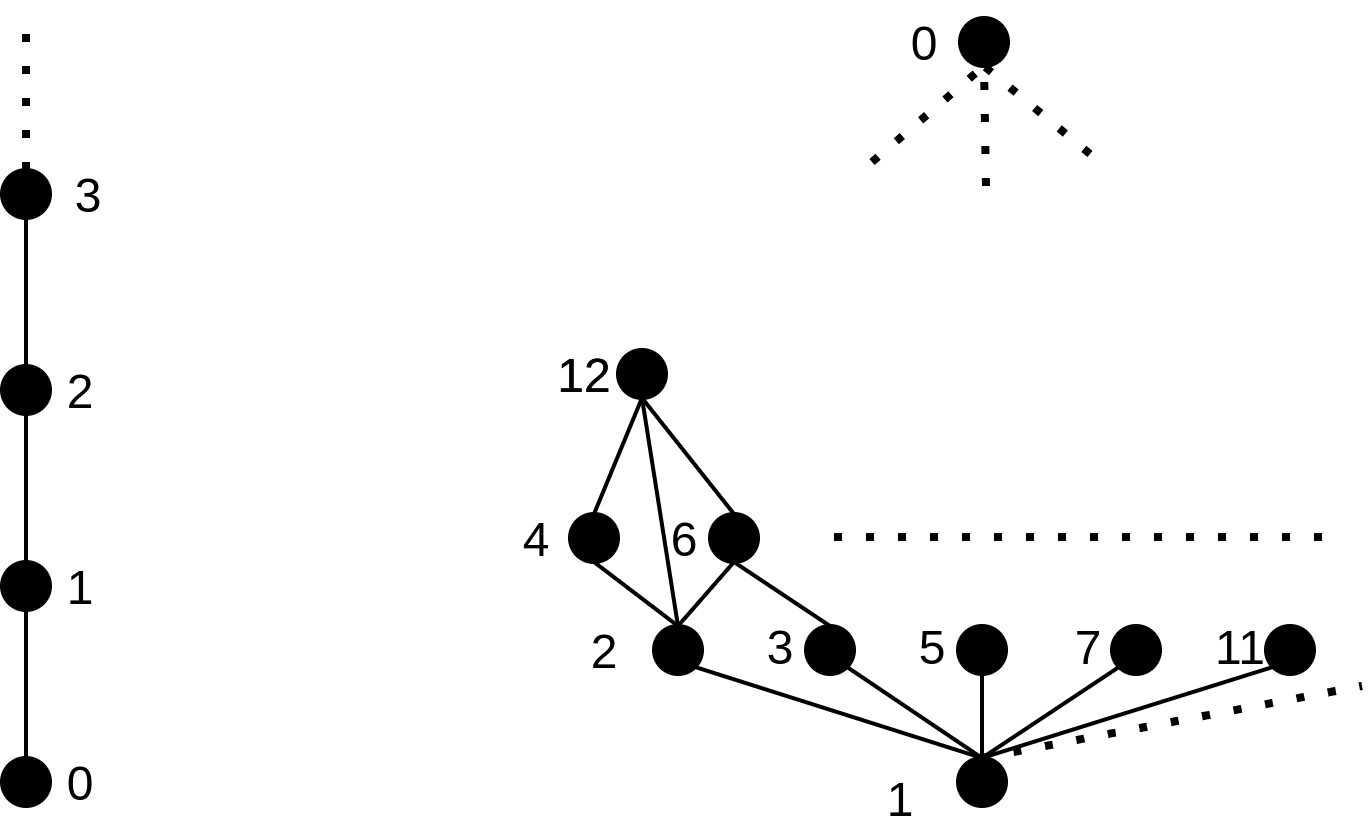
\includegraphics[width=0.5\textwidth]{images/reticolo2.png}
  \caption{Due relazioni d'ordine.}
  \label{figure:relazionireticoli}
\end{figure}
Nella Figure \ref{figure:relazionireticoli} si può vedere una rappresentazione 
(tramite reticoli, definiti a seguire) delle due relazioni d'ordine. 
La prima, quella totale, è rappresentata a destra: si può notare come sia 
``lineare'' a confronto della seconda, parziale, che è rappresentata a 
sinistra: quest'ultima infatti si dirama: alla base ha $1$, il numero che 
divide tutti gli altri; al primo ``strato'' ha tutti i numeri primi, 
il secondo i multipli dei multipli dei numeri primi (che saranno comunque collegati 
ai numeri primi, in quanto saranno divisibili anche per essi) e, commettendo 
un abuso che solitamente viene concesso, in cima vi è il numero $0$ che è divisibile 
da tutti gli altri, benché non sia divisibile per sé stesso. 
Un insieme $P$ con una relazione d'ordine (parziale) $\leq$, 
notato $(P, \leq)$ è detto insieme parzialmente ordinato 
o, in inglese, partially ordered set. Un 
\textbf{reticolo} è un insieme parzialmente ordinato con 
delle proprietà importanti. Un esempio è 
rappresentato in Figura \ref{figure:reticolo}.
\begin{figure}[!h]
  \centering 
  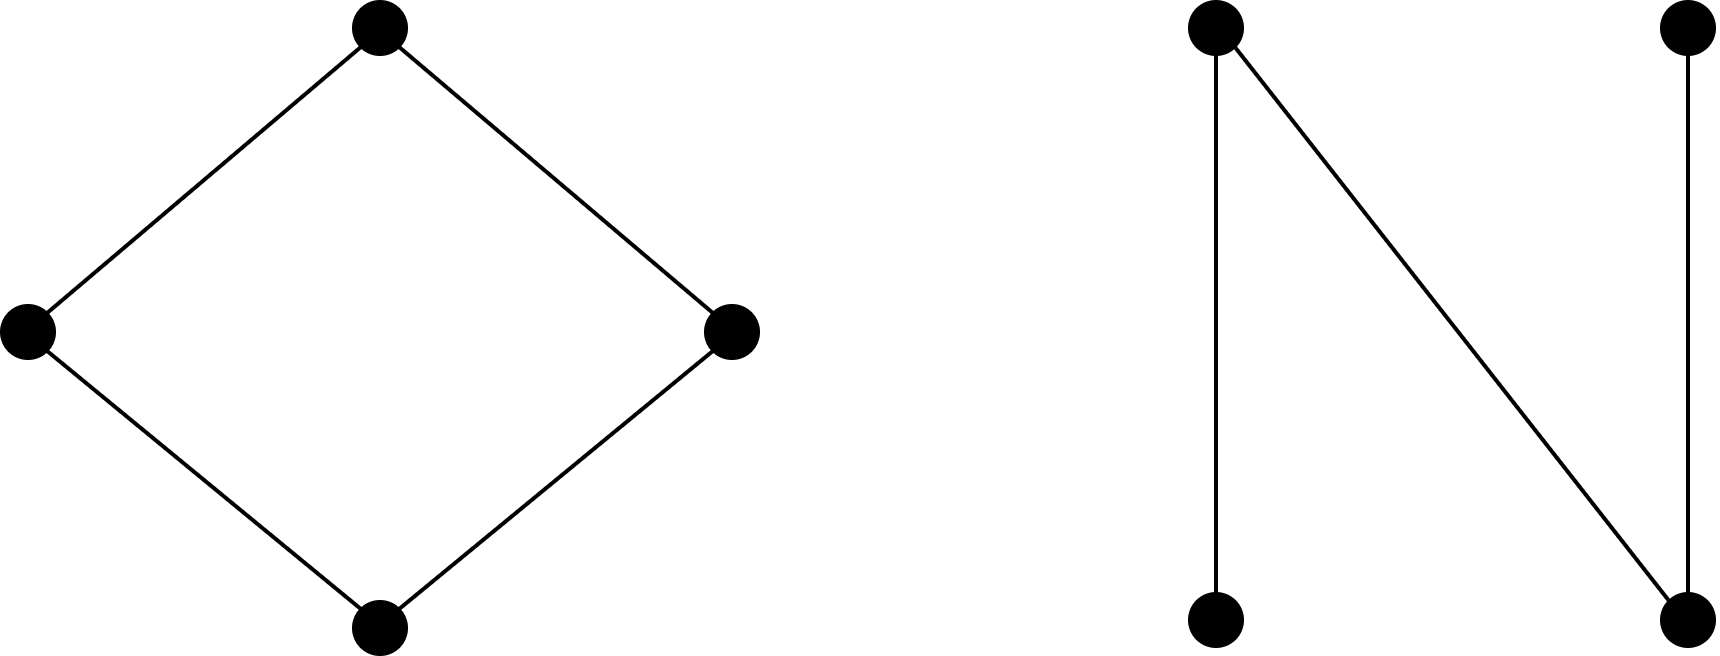
\includegraphics[width=0.5\textwidth]{images/reticolo.png}
  \caption{Due reticoli.}
  \label{figure:reticolo}
\end{figure}
I due reticoli si distinguono perché per uno si possono trovare 
dei valori ``inferiori'' e ``superiori'', 
definiti come 
$$
\inf\{x,y\} = max \{z \in (P, \leq): z \leq x, z \leq y\}
$$
e 
$$
\sup\{x,y\} = min \{ x \in (P, \leq) : z \geq x, z \geq y \}
$$
$S \subseteq P, (P, \leq)$
$$
\inf S = \text{ massimo dei minoranti di } S := \max \{x \in P : z \leq S \forall s \in S \} 
$$ 
$$
\sup S = \min\{ z \in P : z \geq s \forall s \in S \} 
$$ 
e 
$$ 
\max S := z = \sup\{S\} \land z \in S
$$
$$
\min S := z = \inf\{S\} \land z \in S
$$
Un reticolo è un insieme parzialmente ordinato, infatti 
un reticolo $(R, \leq)$ è un \textit{poset} tale che 
per ogni $x, y \in R$ esiste $\inf\{x,y\}$ e $\sup\{x,y\}$. 

\subsection{Struttura Algebrica}
Dato un insieme $S$ e
date le operazioni $*_1, *_2, \cdots, *_n$ delle operazioni 
in $S$, allora $(S, *_i)$ è una \textbf{struttura algebrica}. 
Visto come una struttura algebrica, un reticolo 
è $(R, u, n)$, con $u, n$ operazioni 
$u: R^2 \rightarrow R$ e $ n: R^2 \rightarrow R$, tale che 
le due operazioni siano commutative, associative e 
assorbenti. Ogni reticolo visto come insieme parzialmente 
ordinato è anche una struttura algebrica 
$$
(R, \leq) \iff (R, u, n)
$$
Infatti si può associare una struttura algebrica 
a una struttura ordinata definendo $R\equiv R$, 
$a u b := \inf \{a,b\}$ e $a n b := \sup \{a,b\}$ 
per ogni $a,b \in R$. Si verifichino 
le proprietà di 
commutatività, assorbimento e associatività. 

Si può associare una struttura ordinata 
a ogni struttura algebrica definendo $R \equiv R$ e 
sostanzialmente definendo quando $a \leq b$, ossia 
per ogni $a, b \in R$ si definisce un operatore 
$ a = a n b $ o equivalentemente $b = a u b$. Si deve verificare 
che $a \leq b$ se e solo se $a = a n b$ sia tale 
che $\leq$ sia riflessiva, antisimmetrica e transitiva, 
dalla quale deriva che $R$ è un poset, ma per 
concludere che $R$ sia un reticolo bisogna mostrare 
che per ogni coppia $a,b \in R$ esiste $\inf$ e $\sup$. 
Sia allora $c \leq a$ e $ c \leq b$: bisogna mostrare 
che $c \leq \inf\{a,b\}$, in genere 
$c \leq a n b$. 
Ma $c = a n c = a n (b n c)$ per la definizione di 
$\leq$; si può allora scrivere 
$$
(a n b) n c \iff c \leq a n b 
$$
per definizione di $\leq$. Per il $\sup$ si ragiona 
in modo analogo. 


\subsection{Definizione di Algebra Booleana}
L'algebra booleana è un sistema $(S, n, u, 0, 1, ()^c)$ operazioni 
tali che $(S,n,u)$ sia un reticolo limitato, complementato, 
distribuito e delimitato, ossia: 
\textbf{limitato} in quanto per ogni $a \in S a n 0 = a$ e $a u 1 = a$ ($ a \geq 0$ e $ a \leq 1$); 
\textbf{distributivo} in quanto per ogni $a,b c \in S$ si 
ha $a n (b u c) = (a n b) u (a n c)$ e $a u (b n c) = (a u b) n ( a u c)$; 
\textbf{complementato} in quanto 
$a n a^c = 0$ e $a n a^c = 1$. 
Un esempio è il seguente: dato un insieme $A$ si consideri 
$(P(A), \cup, \cap, \emptyset, A, ()^c)$ e si ha 
$(P(A), \subseteq)$ tale che $A \subseteq B \iff A = A \cap B$. 
Per esercizio, sia $A$ un insieme infinito e sia $F(A)$
l'insieme dei suoi sottoinsiemi finiti o complementi di insiemi 
finiti. Si dimostri che $(F(A), \cup, \cap, \emptyset, A, ()^c)$ è un algebra booleana. Un altro esempio di algebra 
booleana è quella dei valori di verità $(\{0,1\}, \min, \max, 0, 2, 1-\_)$. 

L'algebra delle formule, chiama anche \textbf{Algebra di 
Lindenbaum delle Formule}, è definito $(F_L/\equiv, \land, \lor, \bot, \top, \neg)$. 
Dato che $\equiv$ è una congruenza, si può quindi procedere a definire
$$
A,B \in F_L [A]_{\equiv} \land [B]_{\equiv} = [A \land B]_{\equiv}
$$
$$
A,B \in F_L [A]_{\equiv} \lor [B]_{\equiv} = [A \lor B]_{\equiv}
$$
$$
A,B \in F_L [A]_{\equiv} \rightarrow [B]_{\equiv} = [A \rightarrow B]_{\equiv}
$$
$$
A \in F_L \neg [A]_{\equiv} = [\neg A]_{\equiv}
$$
$$
[\top]_{\equiv} = \text{ tautologie}
$$
$$
[\bot]_{\equiv} = \text{ contraddizioni}
$$
La cardinalità dell'insieme delle classi di equivalenza scrivibili con $n$
variabili è 
$$
|F^{(n)}/\equiv| = 2 ^ {2^n} = |\{F: \{0,1\}^n \rightarrow \{0,1\}\}|
$$

\subsection{Funzioni Termine}
Si immagini, per esempio, di riflettere sul significato di 
$$
\models F \forall \iff \mathfrak{v}: L \rightarrow \{0,1\} \mathfrak{v}(F) = 1
$$
in termini ``computazionali'' significa \textit{tenere fermo} l'argomento 
($F$) e far cambiare le funzioni. Sarebbe comodo scambiare i ruoli, nel 
senso che si vorrebbe che la formula diventasse una funzione, in qualche modo,
e gli assegnamenti degli argomenti. 
Sia ora $A \in F_L$ una formula. Si chiama $Var(A) \subseteq L$ delle lettere 
proposizionali che occorrono in $A$ e $n \in \mathbb{N}$ tale che 
$Var(A) \subseteq \{p_1, p_2, \cdots, p_n\}$.  Sia ora $\hat{A}$ una funzione 
definita come 
$$
\hat{A} : \{0,1\}^n \rightarrow \{0,1\} \text{ tale che } \forall \mathfrak{v}:L \rightarrow \{0,1\}\text{ si ha } \hat{A}(\mathfrak{v}(p_1), \mathfrak{v}(p_1), \cdots, \mathfrak{v}(p_n)) = \mathfrak{v}(A)
$$
la fuzione $\hat{A}$ si chiama \textbf{funzione termine} e, per definirla formalmente, 
si procede per induzione. 
\textbf{caso base:} 
Sia 
$$
A = p_i, p_i \in \{p_1, p_2, \cdots, p_n\}
$$
allora 
$$
\hat{A} := \hat{p_i} : \{0,1\}^n \rightarrow \{0,1\}
$$ 
dove, per ogni $(t_1, \cdots, t_n)$ si ha $\hat{p_i}(t_1, \cdots, t_n) = t_i$, 
ossia l'$i$-esima proiezione. Quindi, per ogni 
$\mathfrak{v}: L \rightarrow \{0,1\} \hat{p_i}(\mathfrak{v}(p_1), \cdots, \mathfrak{v}(p_n)) = \mathfrak{v}(p_i)$. 
\noindent
\textbf{passo induttivo:}
Se $A = \neg B$ allora $\hat{A}(t_1, \cdots, t_n) =  1 - \hat{B}(t_1, \cdots, t_n)$. 
Se $A = B \land C$ allora $\hat{A}(t_1, \cdots, t_n) = min \{\hat{B}(t_1, \cdots, t_n), \hat{C}(t_1, \cdots, t_n)\}$. 
Se $A = B \lor C$ allora $\hat{A}(t_1, \cdots, t_n) = max \{\hat{B}(t_1, \cdots, t_n), \hat{C}(t_1, \cdots, t_n)\}$. 
Se $A = B \rightarrow C$ allora $\hat{A}(t_1, \cdots, t_n) = max \{1 - \hat{B}(t_1, \cdots, t_n), \hat{C}(t_1, \cdots, t_n)\}$. 

E si può riesprimere l'algebra di Lindenbaum come funzioni termine: 
$$
\models F \iff \hat{F}(t_1, \cdots, t_n) = 1 \forall (t_1, \cdots, t_n)
$$
$$
[F]_{\equiv} = [G]_{\equiv} \iff F \equiv G \iff \hat{F} \equiv \hat{G}
$$
e si può riscrivere l'algebra booleana come 
$$
F_L^{(n)} = (\{\hat{F}:\{0,1\}^n \rightarrow \{0,1\}: F \in F_L\}, \land, \lor, \neg, \bot, \top)
$$
dove 
$\hat{B} \land \hat{C} = min \{\hat{B}(t_1, \cdots, t_n), \hat{C}(t_1, \cdots, t_n)\}$
eccetera. 

\subsection{Teorema di Completezza Funzionale}
Per ogni $n$ si ha che l'insieme delle funzioni 
$$
Funz^{(n)} = (\{F: \{0,1\}^{(n)} \rightarrow \{0,1\}\}, \land, \lor, \neg, \bot, \top)
$$
è contenuto in $\hat{F}^{(n)}_L$, 
ossia per ogni $n \in \mathbb{N}$ si ha che per ogni funzione 
$f: \{0,1\}^n \rightarrow \{0,1\}$ esiste ed è costruibile una 
formula $F \in F^{(n)}_L$ tale che $f = \hat{F}$, cioè per ogni 
$(t_1, \cdots, t_n) \in \{0,1\}^n, f(t_1, \cdots, t_n) = \hat{F}(t_1, \cdots, t_n)$. 
Per dimostrarlo, sia data $f: \{0,1\}^n \rightarrow \{0,1\}$. Per un certo 
$n$ si ha che per ogni delle $2^n$ combinazioni si ha un risultato $b_i$, 
con $i$ tra $[0, 2^n -1]$. Si costruisca ora la formula $F$ tale che 
$\hat{F} = f$. Se $b_i = 0 \forall i$, allora $F = \bot$. Altrimenti 
sia $I \subseteq \{0,1,\cdots,2^n-1\}$ tale che $i \in I \iff b_i = 1$, 
ossia l'insieme dei risultati verificati. Per ogni $i \in I$ si consideri l'$i$-esima
della tabella di assegnamenti e risultati 
$a_{i1}, a_{i2}, \cdots, a_{in}$. Per ogni $j \in \{1, \cdots, n\}$ (gli indici delle 
variabili nella riga) si pone 
$$
\begin{cases}
  A_{ij} = p_j \iff a_{ij} = 1 \\
    A_{ij} = \neg p_j \iff a_{ij} = 0
\end{cases}
$$
e, ponendo $F = \lor_{i \in I} \land_{j = 1}^n A_{ij}$
si ha $\hat{F} = f$: basta notare che $\land_{j = 1}^n A_{ij}(t_1, \cdots, t_n) = 1$ 
se e solo se $(t_1, \cdots, t_n) = (a_{i1}, \cdots, a_{in})$. 

Ovviamente $A_{i1} \land A_{i2} \land \cdots \land A_{in}$ valutato sulla riga 
$(a_{i1}, \cdots, a_{in})$ è $1$, dato che $A_{ij}(a_{i1}, \cdots, a_{in}) = a_{ij} $ 
se $a_{ij} = 1$ oppure $A_{ij}(a_{i1}, \cdots, a_{in}) = 1 - a_{ij}$ se 
$a_{ij} = 0$. Sia, ora, $(t_1, \cdots, t_n) \neq (a_{i1}, \cdots, a_{in})$, 
in particolare $t_j \neq a_{ij}$. Allora $A_{ij}(t_1, \cdots, t_n) = 1 - a_{ij}$ 
se $a_{ij} = 1$ e $A_{ij}(t_1, \cdots, t_n) = a_{ij}$ se $a_{ij} = 0$.

Dunque $\land_{j = 1}^{n} A_{ij}) (t_1, \cdots, t_n) = 1$ se $(t_1, \cdots, t_n)$ è 
la riga $i$-esima e, di conseguenza, $F(\lor_{i=I}\land_{j = 1}$ % boh...

\paragraph{Esercizio}
Provare che per ogni $f: \{0,1\}^n \rightarrow \{0,1\}$ esiste una formula 
$G \in F^{(n)}_L$ tale che $\hat{G} = f$. 


\paragraph{Considerazioni sul Teorema di Completezza Funzionale}
Per come è stato provato il Teorema di Completezza Funzionale, la funzione può 
essere espressa 
$$
F = \lor_{i \in I} \land_{j = 1}^{n} A_{ij}
$$
e 
$$
G = \land_{i \in J} \lor_{j = 1}^{n} B_{ij}
$$
e $\hat{F} = F = \hat{G}$ ed è pertanto una dimostrazione dell'esistenza 
delle \textbf{forme normali}. 

Sebbene il Teorema possa sembrare banale in quanto la sua dimostrazione è
semplice, il suo contenuto non è nullo né scontato. Un esempio di mancanza 
funzionale è già presente nella Logica Proposizionale stessa, nonostante 
la dimostrazione precedente rimuovendo il vincolo su $n$, ossia 
$$
Funz^{\omega} := \{f:\{0,1\}^{\omega} \rightarrow \{0,1\}\}
$$
con $\omega = |\mathbb{N}|$, in altre parole l'insieme di tutte le successioni 
infinite di numeri naturali. Se valesse il teorema di completezza funzionale 
anche in questo caso, si dovrebbe poter affermare che tale insieme 
è incluso nelle classi di equivalenza scritte nelle classi di equivalenza 
delle formule scritte con $\omega$ variabili: 
$$
Funz^{\omega} \neg \subseteq \hat{F}^{\omega}_{L} \approx F_L^{\omega}/\equiv
$$
e in particolare 
$$
|Funz^{\omega}| \geq |\mathbb{R}| \geq |\mathbb{N}| = |F_L^{\omega}/\equiv|
$$
Le forme normali che abbiamo trovato non sono desiderabili per gli scopi 
futuri, in quanto sono molto prolisse: ognuno degli $A_{ij}$ menziona 
tutte le lettere proposizionali $p_1, \cdots, p_n$ (analogamente per le 
forme congiuntive) ed è infatti chiamata forma disgiuntica (or di and) 
\textbf{canoniche} o \textbf{complete}. Per esempio, siano date tre variabili 
$p_1$, $p_2$ e $p_3$, si vuole costruire la formula 
$$
F(t_1, t_2, t_3) = t_1
$$
è chiaro che la formula più ``corta'' è $\hat{F} = t_1$, ma con la forma 
canonica il risultato è 
$$
\hat{F} = (p_1 \land \not p_2 \land \not p_3) \lor (p_1 \land \not p_2 \land p_3) \lor (p_1 \land p_2 \land \not p_3) \lor (p_1 \land p_2 \land p_3)
$$
molto più lunga.
\paragraph{Insieme funzionalmente completo di connettivi}
C'è un'altra nozione, legata alla completezza funzionale, che è molto interessante, 
ossia la nozione di \textbf{insieme funzionalmente completo di connettivi}. Un 
insieme $C \subseteq \{\land, \lor, \rightarrow, \neg, \iff, \bot, \top\}$ 
è definito funzionalmente complete se per ogni $F \in F_L$ esiste una $G \in F_L$ 
scritto usando solo i connettivi in $C$ tale che $F \equiv G$ e $\hat{F} = \hat{G}$, 
ossia $[F]_{\equiv} = [G]_{\equiv}$. Un insieme di connettivi funzionalmente 
completo è dato dal teorema di completezza funzionale stesso, ossia 
$C = \{\land, \lor, \neg\}$, che è funzionalmente completeo grazie 
al teorema di completezza funzionale. Si può mostrare facilmente che 
anche $\{\neg, \land\}$ e $\{\neg, \lor\}$ sono completi (in quanto, grazie alle 
leggi di De Morgan, $(A \lor B) = \neg (\neg A \land \neg B)$). Questi non 
sono gli unici insiemi funzionalmente completi: 
$\{\neg, \rightarrow\}$ (in quanto $(A \land B) \equiv \neg (A \rightarrow \neg B)$ 
e $(A \lor B) \equiv ((\neg A) \rightarrow B)$ 
e $\{\rightarrow, \bot\}$. In particolare, un insieme composto da un 
solo connettivo, il \texttt{nand}, è anch'esso funzionalmente completo, 
in quanto ogni altro connettivo è ricostruibile utilizzando solo 
$$
A nand B = \neg (A \land B)
$$
infatti $\neg A \equiv A nand A$ e, ovviamente, $A \land B \equiv \neg ( A nand B)$ 
per definizione. 

\section{Forme Normali}
Le forme normali congiuntive e disgiuntive canoniche (complete) sono 
esageratamente prolisse. Sarebbe utile conservare l'idea delle forme normali 
con formule più succinte. Una terza forma normale, chiamata \textbf{Negation 
Normal Form} (NNF) che, per definizione, è l'insieme delle formule 
che rispettano le seguenti proprietà: 
\begin{description}
  \item non contiene $\rightarrow$ 
  \item $\neg$ occorre solo applicato a lettere proposizionali
\end{description}
quindi, per esempio 
$$ 
p_1 \land \neg(p_2 \lor p_3)
$$
non è una NNF, mentre 
$$
p_1 \land (\neg p_2 \lor \neg p_3)
$$
è una NNF. Ogni formula $F \in F_L$ è equivalente a una $F^{N} \in NNF$. 
Per provare questo, descriviamo come trasformare $F$ in $F^{N}$ in un numero 
finito di passi, dove ogni passo produce una formula equivalente alla precedente. 
Per ottenere la sequenza si applica ad ogni passo una delle seguenti 
trasformazioni: 
\begin{enumerate}
  \item $C \rightarrow D$ in $(\neg C) \land D$
  \item $\neg \neg C$ in $C$
  \item $\neg(C \lor D)$ in $\neg c \land \neg D$
  \item $\neg (C \land D)$ in $\neg C \lor \neg D$
\end{enumerate}
Un'osservazione preliminare su questo algoritmo è che si può mostrare che applicando 
le quattro regole in un ordine qualsiasi si ottiene sempre $F^{N} \in NNF$. 
Si mostrerà che partendo da $(1)$ e applicando le altre trasformazioni si possa 
arrivare a $F^{N}$: sia data $F \in F_L$. In un numero finito di applicazioni 
di $(1)$ si ottiene una $F'$ in IFNF (implication free normal form), equivalente 
a $F$. Questo si misura introducendo una misura di \textit{distanza}: si definisce 
$i(E)$ come il numero di connettivi $\rightarrow$ nella formula $E$. Si ha, quindi, 
che $E \in IFNF \iff i(E) = 0$. Inoltre, se $E \notin IFNF$, allora 
$E'$ ottenuta applicando $(1)$ si ha che $i(E) > i(E')$. 
\`E chiaro che $F \equiv F'$ poiché l'applicazione di $(1)$ è semplicemente 
l'applicazione di una equivalenza eseguita grazie al teorema di sostituzione. 
Quindi, in un certo numero di passi  si ha
$$ 
F = F_0 \equiv \cdots \equiv F' (\in IFNF) \equiv F_i \equiv \cdots \equiv F_n (\in NNF)
$$
e si nota che le applicazioni di $(2)$, $(3)$ e $(4)$ trattano tutte equivalenze logiche. Ciò 
che bisogna dimostrare è che la sequenza di trasformazioni termini, ossia l'algoritmo 
non è infinito. Per dimostrare che l'algoritmo termina, sia ora $A \in F_L$ 
e si definisce 
$$ 
l(A) = \text{ numero di occorrenze di connettivi in } A
$$ 
e 
$$
m(E) = \sum_{\neg A \in E} l(A)
$$
dove la notazione $\neg A \in E$ indica che $\neg A$ sia una sottoformula 

\subsection{Forme Normali Congiuntive}
Le FNC, Forme Normali Congiuntive o CNF, sono un superset delle CNF complete o canoniche.
Un \textbf{letterale} è una formula nella forma $p$ o $\neg p$ per qualche 
lettera proposizionale $p$ - o è una lettera proposizionale o è la sua negata. 
La definizione di \textbf{letterale opposto} a uno dato è, dato $A$ letterale, 
l'opposto di $A$ è
$$
\bar{A} = 
\begin{cases}
  \neg p & A = p \\
  p & A = \neg p
\end{cases}
$$
Una \textbf{clausola} è una disgiunzione di un numero finito di letterali come 
$$
l_1 \lor l_2 \cdots \lor l_k
$$
dove ogni $l_i$ è un letterale. 
Una \textbf{forma normale congiuntiva} è una congiunzione di un numero finito di 
clausole, come 
$$
c_1 \land c_2 \land \cdots \land c_h
$$
dove ogni $c_j$ è una clausola. 
Una \textbf{clausola vuota} $\qedsymbol$ è definita come la disgiunzione 
di zero letterali. Questo concetto è importante e non va confuso col concetto 
di \textbf{CNF vuota} $\emptyset$, definita come la congiunzione di zero clausole, 
poiché prendendo per esempio la sequenza di clausole 
$$
\qedsymbol \\
l_1 \\
l_1 \lor l_2 \\
l_1 \lor l_2 \lor l_3 \\
l_1 \lor l_2 \lor l_3 \lor l_4
$$
ogni assegnamento che soddisfa una formula soddisfa anche la successiva, verso 
il basso - seguendo questa definizione la clausola vuota è insoddisfacibile e 
pertanto, per noi, è $\qedsymbol \equiv \bot$

$$
\emptyset \\
c_1 \\
c_1 \land c_2 \\
c_1 \land c_2 \land c_3\\
c_1 \land c_2 \land c_3 \land c_4
$$
qui, al contrario, ogni assegnamento che soddisfa una clausola soddisfa anche la 
successiva, verso l'alto - seguendo questa definizione la CNF vuota è per 
definizione soddisfacibile ed è, in realtà, soddisfatta da ogni assegnamento 
e $\emptyset \equiv \top$. 

\subsection{Forma Normale Disgiuntiva}
Le FND, Forme Normali Disgiuntive o DNF sono definite come disgiunzione di 
un numero finito di formule 
$$
D_1 \lor D_2 \lor \cdots \lor D_n
$$
dove ogni $D_i$ è una congiunzione chiamata \textbf{co-clausola} di un numero finito 
$$
l_1 \land l_2 \land \cdots \land l_v
$$
di letterali; si tratta, quindi, di una struttura duale rispetto alle CNF. 
Si noti la terminologia speciale per le CNF: questa terminologia è riservata 
alle CNF in quanto la dualità tra CNF e DNG verrà spezzata. 

Ogni formula $F \in F_L$ è logicamente equivalente a una formula $F^c \in CNF$ 
e a una formula $F^d \in DNF$. Questo è già stato dimostrato grazie al teorema 
di completezza funzionale, che tuttavia utilizzava le CNF e DNF complete: una 
versione alternativa della dimostrazione è la seguente, per induzione strutturale 
su $F$. 
\textbf{base induttiva:} se $F = p, p \in L$ allora $p = p^c = p^d$. 
\textbf{passo induttivo:} 
se $F = \neg G$ per ipotesi induttiva si ha $G^c \equiv G$, $G^d \equiv G$ 
e 
\begin{align*}
\neg G^c &= \neg(C_1 \land C_2 \land \cdots \land C_k) \\
       &= \neg C_1 \lor \neg C_2 \lor \cdots \lor \neg C_k) \\
\neg C_i = \neg l_{i1} \land \neg l_{i2} \land \cdots \land \neg l_{ik_i}
\end{align*}
ossia una DNF, inoltre 
$$
\neg G^c \equiv (\bar{l_{11}} \land \bar{l_{12}} \land \cdots \bar{l_{1k_1}}) \lor \cdots \lor (\bar{l_{11}} \land \bar{l_{12}} \land \cdots \bar{l_{1k_n}}) \in DNF
$$
e analogamente per $G^d$ ossia $G^d \in CNF$; si conclude, quindi, che 
$F^c = \neg G^d$ e $F^d = \neg G^c$. 
Se $F = G \land H$ per ipotesi induttiva si hnno $G^c$, $G^d$, $H^c$ e $H^d$; si 
ha $F^c := G^c \land H^c$. Il caso per $F^d$ è più complicato, in quanto 
non si può semplicemente farne la congiunzione ($F^d$ non sarebbe una DNF). 
Si ha, quindi 
$$
(G_1 \lor G_2 \lor \cdots \lor G_n) \land (H_1 \lor H_2 \lor \cdots \lor H_v \equiv \lor_{i,j} (G^d_i \land H^d_j)
$$
che è una DNF. 
Il caso $F=(G \lor H)$ è analogo e si ha $F^d := G^d \lor H^d$ e 
$F^c := \land_{i,j} (G^c_i \lor H^c_j)$.
Il caso $F = (G \rightarrow H)$ si gestisce come $F \equiv (\neg G \lor H)$. 

L'utilizzo della distributività generalizzata non è auspicabile e per dimostrare 
ciò si prenda come esempio la formula 
$$
(p_1 \land q_1) \lor (p_2 \land q_2) \lor (p_3 \land q_3) \in DNF
$$
che è equivalente a 
\begin{align*}
  &\equiv   [p_1 \lor ((p_2 \land q_2) \lor (p_3 \land q_3))] \land [q_1 \lor ((p_2 \land q_2) \lor (p_3 \land q_3))] \\
  & \equiv [p_1 \lor p_2 \land (p_3 \land q_3) \land p_1 \lor q_2 \lor (p_3 \land q_3) \land (q_1 \lor p_2 \lor (p_3 \land q_3) \land q_1 \land q_2 \land (p_3 \lor q_3)] \\
  &\equiv (p_1 \lor p_2 \lor p_3) \land (p_1 \lor p_2 \lor p_3) \land (p_1 \lor q_2 \lor q_3) \land (p_1 \lor q_2 \lor q_3)  \\
  & ~~~~~~ \land (q_1 \lor p_2 \lor p_3) \land (q_1 \lor p_2 \lor q_3) \land (q_1 \lor q_2 \lor p_3) \land (q_1 \lor q_2 \lor q_3)
\end{align*}
come si può notare la lunghezza aumenta notevolmente, e in generale per una DNF
$$
\lor_{i = 1}^{n} (p_i \land q_i)
$$
risulta una CNF 
$$
\land{i = 1}^{2^n}(l_{i1} \lor \cdots \lor l_{in})
$$
ossia un incremento esponenziale. Ripassando ad una DNF si otterrebbero $2^{2^{n}}$ 
formule di lunghezza $n*2^n$ - questo è a causa dell'utilizzo della distributività 
generalizzata. 
Esistono algoritmi più ``furbi'' per creare forme normali? Purtroppo no: la dilatazione 
esponenziale è inevitabile qualsiasi algoritmo venga usato. 

\section{Complessità computazionale}
In questo momento, per decidere se una formula $F \in F_L$ che menziona $n$ lettere 
proposizionali diverse sia soddisfacibile o meno, l'algoritmo che conosciamo
computa la sua tabella di verità, analizzando quindi $2^n$ possibilità, ossia 
un numero esponenziale. Cominciamo definendo cosa sia un problema di 
decisione
\begin{defi}{problema di decisione}
 Dato un alfabeto finito $\Sigma$ e un sottoinsieme non necessariemente 
 finito di stringhe finite  
  $$
 L \subseteq \Sigma^* 
 $$
 il problema di decisione consiste nel affermare se una precisa 
 stringa finita appartenga o meno a $L$, che viene chiamato Linguaggio. 
\end{defi}
dove $\Sigma$ è l'alfabeto finito e $\Sigma^*$ è l'insieme di tutte le 
stringhe di lunghezza finita, chiamate anche \textit{parole}, costruite 
coi simboli di $\Sigma$. 
Ad esempio, fissato 
$$
\Sigma = \{\land, \lor, \neg, \rightarrow, (, ), p, |\}
$$
si possono definire alcuni problemi, per esempio
$$
F_L \subseteq \Sigma ^*
$$
dove il problema risiede nel capire se una certa formula di lunghezza finita
risiede in $F_L$ oppure no. 
Vi sono dei problemi principalmente di natura sintattica, come appunto $F_L$ 
ma anche $NNF$, $CNF$ e $DNF$. Vi sono problemi in cui la natura semantica 
è decisiva, per esempio $SAT$, dove 
$w \in \Sigma^* : w\in SAT \iff w \in F_L \land w \text{ è soddisfacibile}$, 
oppure $TAUT$, dove una stringa finita appartiene a $TAUTO$ se e solo se 
è una formula ed è una tautologia, ossia
$$
w \in \Sigma^* : w \in TAUTO \iff w \in F_L \land \models w
$$
e analogamente $UNSAT$. 


\subsection{Efficienza}
Alcuni dei problemi elencati precedentemente possono essere risolti (decisi) 
in maniera efficiente, ossia data una \textit{parola} $w$ decidere se 
appartiene ad un certo linguaggio: esempi di soluzioni efficienti sono 
quelle che riguardano tutti i problemi sintattici, risolvibili in tempo 
al massimo quadratico e in realta anche lineare con tecniche di parsing. 

I problemi che riguardano la semantica, invece, sono tipicamente più complessi
da risolvere e infatti, per quanto conosciamo fino ad ora, si possono risolvere 
solo (nel caso peggiore) con un analisi dell'intera tabella di verità della 
formula, quindi con un numero esponenziale di calcoli. \`E importante rimarcare 
nuovamente che benché sussista questa difficoltà, verificare che 
un singolo assegnamento verifichi la formula è invece un calcolo semplice 
che richiede un tempo decisamente più contenuto rispetto al problema di 
decidibilità.

Quindi, vi sono dei problemi decidibili efficientemente, 
dei problemi decidibili molto difficilmente e verificabili facilmente 
e dei problemi decidibili molto difficilmente e verificabili difficilmente; 
da qui parte una gerarchia di classi di complessità infinita, ma a noi interesseranno 
solo le prime due. 
 
Per essere più precisi, si fissa un modello astratto di computazione, che fornisca 
la nozione di \textit{passo elementare}, in modo da poter ragionare precisamente 
sull'efficienza dei problemi. 
Qualunque modello di computazione che costituisca un modello realistico 
di calcolatore, con associata una nozione di passo elementare per costruire 
algoritmi, classifica i problemi nello stesso modo. 

\begin{oss}[Tesi di Church-Turing]
  Ogni modello ragionevole di computazione è equivalente.
\end{oss}

Uno dei modelli di computazione è quello delle Macchine di Turing (MdT): un'idea 
della Macchina di Turing è immaginarla come una macchina che lavora su un 
nastro infinito in lettura e scrittura, mantenendo uno stato e operando su 
una singola porzione di nasto in lettura utilizzando un programma per 
muoversi tra gli stati e scrivere sul nastro. 

Si può passare ora alla definizione formale delle classi dei problemi: 
\begin{defi}[Classe $\mathbb{P}$]
  La classe dei problemi ``efficientemente decidibili'' è definita, con una 
  certa ideologia sottesa, come tutti quei problemi che possono essere 
  risolti in tempo polinomiale, ossia esiste una certa Macchina di Turint T 
  e un polinomio $p: \mathbb{N}\rightarrow \mathbb{N}$ per i quali per ogni 
  $w \in \Sigma^*$  la computazione della MdT sull'input $w$, 
  denotato $T(w)$ termina entro $p(||w||)$ passi e per ogni $w \in L$ si 
  ha che $T(w)$ accetta il problema e per ogni $w \notin L$  si ha 
  che $T(w)$ non accetta, ossia risolve il problema.
\end{defi}

\begin{defi}[Classe $\mathbb{NP}$]
  La classe dei problemi ``verificabili efficientemente'' è definita come 
  tutti quei problemi tali per cui esiste una Macchina di Turing deterministica 
  e due polinomi $p,q:\mathbb{N}\rightarrow \mathbb{N}$ tali che per ogni 
  $w \in \Sigma^*$ e ogni $z \in \Gamma^*$, ossia un \textbf{certificato}, 
  che si può immaginare proddotto oracolarmente, si ha 
  che $T(w,z)$ termina entro $p(||w||)$ passi e si ha che per ogni 
  $w \in L$ esiste $z \in \Gamma^*$ tale che $||z|| \leq q(||w||)$ (ossia 
  il certificato è sufficientemente corto) e $T(w,z)$ accetta e per ogni 
  $w \notin L$ si ha che ogni possibile $z \in \Gamma^*$ sufficientemente corto
  si ha che $T(w)$ rifiuta.
\end{defi}

\begin{defi}[Riducibilità]
        Un problema $L_1 \subseteq \Sigma^*$ è \textbf{riducibile in tempo polinomiale} 
        a un altro problema $L_2 \subseteq \Gamma^*$ se e solo se esistono
        una Macchina di Turing $T_{{L_1}, {L_2}}$ e un polinomio
        $p: \mathbb{N} \rightarrow \mathbb{N}$ tale che per ogni $w \in L_1$
        $T(w)$ trasfroma $w$ in $w' \in \Gamma^*$ in un numero di passi 
        minore o uguale a $p(||w||)$. 
\end{defi}

Per indicare la relazione di riducibilità tra due problemi si indica la notazione 
$L_1 \preceq_p L_2$ per indicare che il primo problema è riducibile polinomialmente 
al secondo; la nozione di riducibilità è utile poiché rende possibile risolvere 
istanze del problema $L_1$ ``riscrivendole'' come se fossero istanze di $L_2$
(chiaramente questa utilità si verifica quando è più facile risolvere $L_2$ di 
$L_1$). 
Un esempio di riducibilità polinomiale è 
$$
TAUTO \preceq_p UNSAT
$$
poiché la trasformazione $w \rightarrow \neg w$ è semplice e si sa che 
$w$ è tautologica se e solo se $\neg w$ è insoddisfacibile.

\begin{defi}[Problemi $\mathbb{NP}$-completi]
        Un problema appartenente alla classe $\mathbb{NP}_c$ è un problema 
        $L \subseteq \Sigma^*$ se e solo se 
        \begin{itemize}
                \item $L \in \mathbb{NP}$
                \item ogni $L' \in \mathbb{NP}$ è tale che $L' \preceq_p L$ 
        \end{itemize}
        La seconda proprietà si chiama $\mathbb{NP}$-hardness. 
\end{defi}
Come corollario della definizione dei problemi $\mathbb{NP}_c$, si ha che risolvendo 
polinomialmente un problema di tale classe si dimostra che 
$$
\mathbb{P} = \mathbb{NP}
$$

\begin{teo}[di Cook-Levin]
        $CNFSAT \in \mathbb{NP}$
\end{teo}

Per dimostrare che $CNFSAT \preceq SAT$, basta realizzare che una formula 
in CNF è comunque ancora una formula e pertanto la trasformazione è ovviamente 
polinomiale, essendo la funzione identità. Dimostrare che $SAT \preceq CNFSAT$ 
è tutt'altra questione benché sia ovvio dal Teorema di Cook; tuttavia, questa 
proprietà che invece non vale per le DNF, ossia $SAT \npreceq DNFSAT$, è una 
buona motivazione per concentrarsi sulle CNF. 
Si mostra ora, esplicitamente, che SAT si riduce polinomialmente a CNFSAT, 
conservando non l'equivalenza logica ma la relazione di equisoddisfacibilità. 

\subsection{Equisoddisfacibilità}
\begin{defi}[Equisoddisfacibilità]
        Siano $A, B \in F_L$. Le due formule sono equisoddisfacibili se e solo 
        se $A$ è soddisfacibile se e solo se $B$ è soddisfacibile, ossia 
        se $A$ e $B$ sono entrambe soddisfsacibili o entrambe insoddisfacibili. 
\end{defi}

\subsubsection{Esempi}
\paragraph{1}
Date le due formule $\neg (A \land B)$ e $\neg A \lor \neg B$, è noto 
che sono equivalenti grazie alle leggi di De Morgan e sono, di conseguenza, 
anche equisoddisfacibili.
\paragraph{2} $\neg (A \land B)$ e $(\neg A \land \neg B)$ non sono equivalenti, 
infatti l'assegnamento $A=1$ e $B=1$ soddisfa solo una delle due, tuttavia 
sono equisoddisfacibili.
\paragraph{3} $A \land \neg A$ e $\neg A \neg B$ non sono né equivalenti né
equisoddisfacibili.

Da questi esempi si può chiaramente notare che l'equivalenza implica l'equisoddisfacibilità 
mentre il contrario non è affatto verificato.

\paragraph{4}
L'equisoddisfacibilità è un tipo di relazione d'equivalenza, in quanto 
valgono le proprietà di simmetria, transitività e riflessività.
\paragraph{5} L'equisoddisfacibilità è una congruenza rispetto ai 
connettivi, pensati come operazioni? Non lo è. Sia, per esempio 
$\models A$, quindi $A \in [\top]$ e $B$ soddisfacibile ma non tautologica; 
sono equisoddisfacibili, in quanto sono entrambi chiaramente soddisfacibili. 
Se fosse una congruenza, rispetto alle varie operazioni l'equisoddisfacibilità 
dovrebbe essere mantenuta, invece $\neg A$ è $\bot$, mentre $\neg B$ è 
ancora soddisfacibile, pertanto non sono equisoddisfacibili.

\paragraph{6} Le classi di equivalenza delle formule, per esempio su 
due variabili, sono costruite nelle forme come $F_L^{(2)}/\equiv$, ossia 
$16$ diverse classi ($2^{2^2}$). Per l'equisoddisfacibilità vi saranno unicamente 
due classi, ossia l'insieme delle formule insoddisfacibili ($[\bot]$) e 
tutte le rimanenti, ossia tutte quelle almeno soddisfacibili.  

\subsection{Riduzione $SAT \preceq CNFSAT$}
Sia $A \in F_L$ tale che $A$ sia in Negation Normal Form, ossia $A \in NNF$. 
Se $A \notin CNF$, allora contiene almeno una sottoformula del tipo 
$C \lor (D_1 \land D_2)$ oppure $(D_1 \land D_2) \lor C)$. Questo si dimostra 
semplicemente confermando che $A \in NNF$ ma non $A \in CNF$, quindi la parte 
che non rispetta la CNF deve essere una disgiunzione di congiunzioni. Trattiamo, 
d'ora in poi, solo il primo dei due casi, ossia quello in cui nella formula 
appare la sottoformula $C \lor (D_1 \land D_2)$, senza perdita di generalità.
Sia data $A \in NNF$ e sia $B = C \lor (D_1 \land D_2)$ una sua violazione; 
per ogni violazione si introduce una nuova lettera proposizionale $a \in L$ che 
ancora non è presente in $A$. 
Si definisce ora 
$$
B' := B[a/D_1 \land D_2] \land (\neg a \lor D_1) \land (\neg a \lor D_2)
$$
dove 
$$
B'' := B[a/D_1\land D_2]
$$
è la formula ottenuta rimpiazzando ogni occorrenza di $D_1 \land D_2$ con $a$ 
in $B$. 
Come prima osservazione, si ha che $(\neg a \lor D_1) \land (\neg a \lor D_2)$ 
è equivalente a $a \rightarrow (D_1 \land D_2)$. 
Si mostra che $B'$ e $B$ sono equisoddisfacibili, ma in genere non 
sono equivalenti: 
\begin{proof}[$B \in SAT \rightarrow B' \in SAT$]
        Per ipotesi, dato che $B$ è soddisfacibile, sia $\mathfrak{v}:L \rightarrow \{0,1\}$
        tale che $\mathfrak{v}(B) = 1$, ossia $\mathfrak{v} \models B$. 
        Si definisce 
        $$
        \mathfrak{v}_a: L \rightarrow \{0,1\} = 
        \begin{cases}
                \mathfrak{v}_a(p) = \mathfrak{v}(p) & \forall p \in L, p \neq a \\
                \mathfrak{v}_a(a) = \mathfrak{v}(D_1 \land D_2) 
        \end{cases} 
        $$
        L'assegnamento $\mathfrak{v}(a)$ è ben definito, nel senso che non 
        da alla stessa lettera proposizionale due assegnamenti diversi.
        Si nota che $\mathfrak{v}_a \models a \rightarrow (D_1 \land D_2)$, 
        dato che per definizione $\mathfrak{v}_a(a) = \mathfrak{v}(D_1 \land D_2)$
        e per interpretazione dell'implicazione $0 \rightarrow 0 = 1$ e 
        $1 \rightarrow 1 = 1$; dunque, $\mathfrak{v}_a(B') = \mathfrak{v}_a(B'')$, 
        in quanto la ``coda'' di $B'$, ossia $(\neg a \lor D_1) \land (\neg a \lor D_2)$, 
        ha un assegnamento uguale a $1$, ossia 
        $\mathfrak{v}_a(B') = \mathfrak{v}_a(B'') \land 1$.

        $B$ si può riscrivere come 
        $$
        B = B''[D_1 \land D_2/a]
        $$
        dato che $a$ non appare in $B$, e quindi 
        $$
        B'' = (B[a/D_1 \land D_2])[a/a]
        $$
        e grazie al Lemma di Sostituzione si può affermare che i due valori 
        di verità di $B$ e $B''$ sono uguali in quanto i valori di verità di $a$ 
        e $D_1 \land D_2$ sono uguali. Ora si può scrivere 
        \begin{align*}
                1 &= \mathfrak{v}(B) \text{ per ipotesi } \\
                  &= \mathfrak{v}_a(B) \text { poiché } a \text{ non occore in } B \\
                  &= \mathfrak{v}_a(B'') \text{ per il lemma di sostituzione}  \\
                  &= \mathfrak{v}_a(B') 
        \end{align*}
        ossia l'assegnamento che soddisfa $B$ soddisfa anche $B'$, ossia 
        sono equisoddisfacibili. 
\end{proof}
\begin{proof}[$B' \in SAT \rightarrow B \in SAT$]
        La sequenza di derivazioni utilizzata per la dimostrazione precedente 
        è ancora buona, tuttavia c'è un vincolo all'inizio, 
        ossia l'assunzione che se $\mathfrak{v}(B) = 1$ allora $\mathfrak{v}_a(B) = 1$; 
        per definizione 
        $$
        \mathfrak{v}_a: L \rightarrow \{0,1\} = 
        \begin{cases}
                \mathfrak{v}_a(p) = \mathfrak{v}(p) & \forall p \in L, p \neq a \\
                \mathfrak{v}_a(a) = \mathfrak{v}(D_1 \land D_2) 
        \end{cases} 
        $$
        che non è la stessa cosa di dire che $B'$ è soddisfacibile, 
        ossia $\mathfrak{v}_a \models B'$, poiché $B'$ potrebbe essere soddisfatto 
        da assegnamenti che non sono nella forma $\mathfrak{v}_a$. Il ragionamento 
        è un po' più complicato. 

        Si supponga che $B'$ sia soddisfacibile da un assegnamento della forma 
        $\mathfrak{v}_a$, ossia tale che $\mathfrak{v}_a(a) = \mathfrak{v}(D_1 \land D_2)$; 
        allora, in questo caso si può tranquillamente ribaltare la catena di uguaglianze 
        precedente: 
        \begin{align*}
                1 &= \mathfrak{v}_a(B') \\
                  &= \mathfrak{v}_a(B'') \text{ per il lemma di sostituzione}  \\
                  &= \mathfrak{v}_a(B) \text { poiché } a \text{ non occore in } B 
        \end{align*}
        dunque $\mathfrak{v}_a \models B$. 
        Si supponga, ora, che $B'$ sia soddisfatto solo da assegnamenti 
        $\mathfrak{w}$ che non sono della forma $\mathfrak{v}_a$, 
        ossia $\mathfrak{w}(a) \neq \mathfrak{v}(D_1 \land D_2)$. 
        Vi sono allora due casi: nel primo $\mathfrak{w}(a)= 0 \neq \mathfrak{v}(D_1 \land D_2) =  1$, 
        nel secondo accade il contrario, ossia 
        $\mathfrak{w}(a) = 1 \neq \mathfrak{v}(D_1 \land D_2) = 0$ tuttavia 
        quest'ultimo caso è impossibile, poiché 
        $\mathfrak{w}(a \rightarrow D_1 \land D_2) = \mathfrak{w}(1 \rightarrow 0) = 0$
        e quindi non può soddisfare $B'$. Quindi rimane 
        il primo caso e bisogna mostrare che anche 
        tale assegnamento effettivamente soddisfa $B'$ e non è un assurdo; come 
        informazione di carattere generale utile per risolvere 
        questo problema, sia E un'espressione formata solo da $0, 1, \land, \lor$ 
        interpretati come $\min$ e $\max$. Il valore di $E$ è $0$ o $1$. 
        Sia $E'$ ottenuta da $E$ rimpiazzando nessuna o più occorrenze 
        del simbolo $0$ con $1$. Allora $E \leq E'$. Questo si dimostra 
        affermando che $0, 1, \min, \max$ sono tutte funzioni 
        non decrescenti e $E$ ed $E'$ sono composizioni di funzioni 
        non decrescenti, pertanto sono non decrescenti (un'altra prova è 
        per induzione strutturale su $E$).

        Ora, tornando al problema principale, si ha che  $\mathfrak{w}(B') = 1$, 
        $\mathfrak{w}(a) = 0$ e $\mathfrak{w}(D_1 \land D_2) = 1$. Dato 
        che la formula iniziale era in $NNF$, anche $B'$ e $B$ sono in 
        NNF. Dunque, considerando $\mathfrak{w}(B)$ e $\mathfrak{w}(B'')$ 
        si possono esprimere entrambe come funzioni termine 
        di $B''$, ossia  
        $$
        \hat{B}''(\mathfrak{w}(p_1), \cdots, \mathfrak{w}(p_n), \mathfrak{w}(D_1 \land D_2))
        $$
        e
        $$
        \hat{B}''(\mathfrak{w}(p_1), \cdots, \mathfrak{w}(p_n), \mathfrak{w}(a))
        $$
        rispettivamente. Come prima osservazione, $\mathfrak{w}(B'')$ e $\mathfrak{w}(B)$
        sono considerabili come espressioni costruite su $0,1,\land,\lor$, poiché 
        sono entrambi in $NNF$. Si può concludere, quindi, che 
        $$
        \mathfrak{w}(B'') \leq \mathfrak{w}(B) \rightarrow 1 \leq \mathfrak{w}(B) \rightarrow \mathfrak{w}(B) = 1
        $$
        applicando le sostituzioni sui valori di verità di $a$ e $D_1 \land D_2$. 
\end{proof}

\begin{oss}[Nota finale]
        Si sarebbe potuto definire $B'$, alternativamente, come segue: 
        \begin{align*}
                B' &:= B[a/D_1 \land D_2] \land (a \iff (D_1 \land D_2))^c \\
                   &=  B[a/D_1 \land D_2] \land (\neg a \lor D_1) \land (\neg A \lor D_2) \land ((D_1 \land D_2) \rightarrow a)^c \\
                   &=  B[a/D_1 \land D_2] \land (\neg a \lor D_1) \land (\neg A \lor D_2) \land (a \lor \neg D_1 \lor \neg D_2)
        \end{align*}
        Adottando tale definizione per $B'$, allora nella prova che $B'$ soddisfacibile 
        implica $B$ soddisfacibile si sarebbe potuto mostrare che $B'$ è 
        soddisfatto solo da assegnamenti nella forma $\mathfrak{v}_a$, 
        ossia $\mathfrak{v}_a(a) = \mathfrak{v}(D_1\land D_2)$.
\end{oss}

Nel passaggio da $B$ a $B'$ si osserva una dilatazione nella lunghezza della 
formula, ossia $B'$ è \textit{più lungo} di $B$; data la formula 
generale 
$$
B' \rightarrow B[a/D_1 \land D_2] \land (\neg a \lor D_1) \land (\neg a \lor D_2)
$$
la parte della formula $B$ viene al massimo accorciata, però sia aggiunge una 
decina di simboli: si può affermare che la lunghezza di 
$B'$ sia $|B'| = |B| + k$, con $k$ una costante dipendente dal 
modo in cui si conta la lunghezza (si contano le parentesi come simboli eccetera). 
Per ogni ``violazione'' nella formula originale, la formula risultante equisoddisfacibile
senza tale violazione è più lunga di $k$ caratteri e, se vi sono $v$ violazioni, 
dopo $v$ passi la formula risultante sarà CNF e avrà lunghezza $|B| + v * k$, 
non esponenziale rispetto alla lunghezza iniziale. 

La tecnica usata per ridurre $SAT \preceq_p CNFSAT$ che consiste nel rimpiazzare 
$B$ con $B'$ equisoddisfacibile è ispirata alla riduzione 
$$
SAT \preceq 3CNFSAT
$$
dovuta a Karp. Il passaggio $B \rightarrow B'$ è un esempio del cosiddetto 
``Tseytin's Trick'', che si usa per ridurre $F \in F_L$ a una 
in $3CNFSAT$ ad essa equisoddisfacibile. 

\begin{defi}[Problemi $3CNFSAT$]
        $3CNFSAT \subseteq CNFSAT \subseteq F_L$ è costituito da tutte 
        e sole le CNF dove ogni clausola contiene o esattamente $3$ 
        letterali. $3CNFSAT \in \mathbb{NP}$ ed è addirittura $\mathbb{NP}$-completo.
\end{defi}
\begin{oss}[Problemi $2CNFSAT$]
        $2CNFSAT \in \mathbb{P}$.
\end{oss}
\subsubsection{Algoritmo di riduzione a CNF equisoddisfacibili}
Sia data $F \in F_L$ e sia $A \in NNF$ $A \equiv F$, che si 
ottiene in tempo polinomiale rispetto alla lunghezza di $F$. 
Se $A \in CNF$, allora l'algoritmo termina, altrimenti è necessario 
individuare la violazione $B$ sottoformula di $A$ e si sostituisce con 
$B'$ e si ritorna al check su $A \in CNF$. 
\subsubsection{Esempi}
\paragraph{1} Sia $A := p \lor (q \land r)$. Si trasforma ora in una 
formula equisoddisfacibile in CNF: 
$$
A' := (p \lor a) \land (\neg a \lor q) \land (\neg a \lor r)
$$
Queste due formule non sono equivalenti, infatti vi sono assegnamenti 
che portano a risultati diversi; tuttavia sono equisoddisfacibili.

\paragraph{2} 
Sia $A := (p_1 \land p_2) \lor (p_2 \land q_2) \lor (p_3 \land q_3)$. Si 
ha $A'$ uguale a 
\[
        ((p_1 \land q_1) \lor (p_2 \land q_2) \lor a_3) \land (\neg a_2 \lor p_3) \land (\neg a_3 \lor q_3)
\]
e, applicando di nuovo la trasformazione, si ottiene 
\[
        ((p_1 \land q_1) \lor a_2 \lor a_3) \land (\neg a_3 \lor p_3) \land (\neg a_3 \lor q_3) \land (\neg a_2 \lor p_2) \land (\neg a_2 \lor p_2) 
\]
e si conclude definendo $A'''$
\[
(a_1 \lor a_2 \lor a_3) \land (\neg a_3 \lor p_3) \land (\neg a_3 \lor q_3) \land (\neg a_2 \lor p_2) \land (\neg a_2 \lor q_2) \land (\neg a_1 \lor p_1) \land (\neg a_1 \lor q_1)
\]
Data una formula con $n$ letterali si generano $2*n +1 $ clausole, 
di cui una con $n$ letterali e $2n$ con due letterali, laddove utilizzando la 
distributività se ne generavano $2^n$ ognuna con $n$ letterali. 


\section{Deduzione Automatica}
Vogliamo studiare i problemi $CNFSAT$, che è $\mathbb{NP}$-completo, e 
il suo complemento $CNFUNSAT$, che è un problema $\mathbb{NP}$-completo, 
in quanto la riduzione polinomiale $SAT \preceq_p CNFSAT$ e pertanto 
studiare $CNFSAT$ è uguale a studiare $SAT$. Analogamente si può studiare 
$TAUTO \preceq_p SAT^c \preceq_p CNFUNSAT$. In realtà siamo nella posizione 
di studiare $\Gamma \models A$ tramite la risoluzione di $CNFSAT$ e $CNFUNSAT$
Il motivo per cui non studiare invece $DNFSAT$ e $DNFUNSAT$ è che non 
c'è un algoritmo per ``tradurre'' una formula arbitraria equisoddisfacibile 
in DNF in modo che sia sufficientemente corta: i metodi conosciuti allungano
esponenzialmente la formula. 

\begin{defi}[Variazione notazionale]
        Date $F_i \in F_L$ si possono descrivere le formule 
        $$
        F_1 \land F_2 \land \cdots \land F_k
        $$
        e 
        $$
        F_1 \lor F_2 \lor \cdots \lor F_k
        $$
        si possono scrivere senza formule grazie all'associatività, 
        e inoltre le formule nelle rispettive formule si possono 
        scambiare ($F_1 \land F_2 \equiv F_2 \land F_1$) grazie 
        alla commutatività e si possono espandere le singole formule 
        ($F_1 \land F_1  \equiv F_1$) grazie all'idempotenza. 

        In questo frangente si possono anche ``tralasciare'' gli operatori 
        $\land$ e $\lor$, chiaramente nel caso in cui ci sia un utilizzo uniforme. 
        La notazione può diventare puramente insiemistica, ossia 
        $$
        \{F_1, F_2, \cdots, F_k\}
        $$
        per indicare entrambe le formule, specificando il connettivo che le 
        unisce. D'ora in poi una CNF sarò un \textbf{insieme} di clausole, 
        dove ogni clausola sarà un insieme di letterali. 
        Per esempio 
        $$
        (p \lor q \lor \neg r) \land (q \lor r \lor a) \land p
        $$
        diventa 
        $$
        \{ \{p, q, \neg r\}, \{q, r, a\}, \{p\}\}
        $$
        ossia una CNF in forma insiemistica, che contiene clausole in 
        forma insiemistica. 
        Una teoria costruita da CNF è l'insieme di tutte le clausole appartenenti 
        a qualche CNF della teoria. 
        La CNF vuota è $\emptyset$, mentre la clausola vuota $\qedsymbol$ 
        e la CNF che contiene la clausola vuota avrà la forma 
        $\{\cdots, \qedsymbol, \cdots \}$.
\end{defi}

Il problema della conseguenza logica di una teoria 
$$
\Gamma \models A
$$
si può ridurre a calcolare la soddisfacibilità di 
$$
S := 
$$
Si è quindi ridotto il problema $\Gamma \models A$ al problema $S \in SAT$,
dove $S$ è un insieme di clausole considerate come insiemi di letterali, 
eventualmente infinito. 


\subsection{Metodi refutazionali}
$S$ è soddisfacibile se esiste $\mathfrak{v}:L \rightarrow \{0,1\}$ tale 
che $\mathfrak{v} \models c$ per ogni clausola $c \in S$, in altre parole 
in ogni $c \in S$ esiste un letterale $l \in c$ tale che $\mathfrak{v} \models l$. 
Se l'obiettivo è dimostrare che $S$ è soddisfacibile, una strategia 
può essere ampliare $S$ in un nuovo insieme $S \subseteq S'$ in modo 
tale che $S'$ è equivalente o almeno equisoddisfacibile a $S$.
Ad esempio, se ampliando iterativamente $S$ in $S'$, $S''$ fino a $S^{(u)}$ 
e alla fine la clausola vuota appartiene a $S^{(u)}$ allora quest'ultimo 
è insoddisfacibile, e quindi anche $S$ lo è. Questa idea può essere sfruttata 
disegnando \textbf{metodi refutazionali}, ossia metodi che hanno l'obiettivo di 
provare l'insoddisfacibilità di un insieme di clausole, in questo frangente, 
ma più in generale anche di una formula o una teoria, i quali sono basati 
sulla regola di inferenza chiamata \textbf{principio di risoluzione}, 
il quale è utile per un tipo di calcolo particolarmente adatto a essere automatizzato, 
ossia SAT solver e Theorem Prover. 

\begin{defi}[Principio di Risoluzione]
        Date due clausole $C_1$ e $C_2$ si dice che $D$ è la risolvente 
        di $C_1$ e $C_2$ sul pivot $\ell$ un letterale se e solo se
        \begin{itemize}
                \item $\ell \in C_1$
                \item $\bar{\ell} \in C_2$
                \item $D := ((C_1 \setminus \{\ell\}) \cup (C_2 \setminus \{\bar{\ell}\})$
        \end{itemize}
       e si scriverà $D = \mathbb{R}(C_1,C_2; \ell, \bar{\ell})$. 
\end{defi}

\subsubsection{Esercizio}
Mostrare che $(C_1 \setminus \{\ell\}) \cup (C_2 \setminus \{\bar{\ell}\})$ può essere 
diverso da $(C_1 \cup C_2) \setminus \{\ell, \bar{\ell}\}$

\subsubsection{Esempio}
Sia $C_1 := \{x, y, \neg t\}$ e $C_2 := \{u, \neg y, t\}$; 
si ha $D_1 = \mathbb{R}(C_1, C_2; y, \neg y) = \{x, \neg t, u\}$ e 
$D_2 = \mathbb{R}(C_1, C_2; \neg t, t) = \{x, y, y\}$. 

\begin{lem}[di correttezza di $\mathbb{R}$]
        Sia $D = \mathbb{R}(C_1, C_2; \ell, \bar{\ell})$, allora 
        $$
        \{C_1, C_2\} \models D
        $$
\end{lem}

\begin{proof}
        Bisogna dimostrare che ogni $\mathfrak{v}$ tale che $\mathfrak{v} \models C_1$ 
        e $\mathfrak{v} \models C_2$ implica $\mathfrak{v} \models D$. Sia allora 
        $\mathfrak{v}$ tale che $\mathfrak{v} \models C_1$ 
        e $\mathfrak{v} \models C_2$, allora $\mathfrak{v} \models m$ e 
        $\mathfrak{v} \models n$ per due letterali $m \in C_1$ e $n \in C_2$; 
        se fosse il caso che $m = \ell$ e  $n = \bar{\ell}$ allora 
        $\mathfrak{v}(\ell) = 1$ e $\mathfrak{v}(\ell) = 0$, impossibile. 
        Allora,almeno uno tra $m$ e $n$ è tale che $m \neq \ell$ o $n \neq \ell$ 
        e assumendo senza perdita di generalità $m \neq l$ si ha 
        $m \in D$, dunque $\mathfrak{v}(D) = 1$. 
\end{proof}

\begin{cor}
        Se $\mathbb{R}(C_1, C_2; \ell, \bar{\ell}) = \qedsymbol$ allora 
        $\{C_1, C_2\}$ è insoddisfacibile, in quanto $\{C_1, C_2\} \models \qedsymbol$.
\end{cor}
\begin{cor}
        Sia $S$ un insieme di clausole e sia $S := S_0, S_1, \cdots, S_k$ una 
        successione di insiemi tale che per ogni $i = 0, \cdots, k-1$ 
        si ha che $S_{i+1}$ si ottiene unendo a $S_i$ una o più risolventi 
        di clausole in $S_i$ e che $\qedsymbol \in S_k$, quindi $S$ è 
        insoddisfacibile.
\end{cor}
L'obiettivo è mostare che i calcoli refutazionali basato su applicazioni 
ripetute della risoluzione sono corretti e completi (refutazionalmente).
In genere, per un calcolo logico si studiano infatti le due
seguenti proprietà:
\begin{defi}[Correttezza]
        Un calcolo si definisce \textbf{corretto} se i certificati che produce 
        testimoniano il vero, ossia sono corretti, in altre parole 
        non produce certificati fasulli. Per esempio, nel frangente attuale 
        $S_0, S_1, \cdots, S_k \ni \qedsymbol$ è un certificato 
        corretto dell'insoddisfacibilità di $S = S_0$. 
\end{defi}
\begin{defi}[Completezza]
        Un calcolo è completo se non omette alcun certificato. Nella situazione 
        attuale vuol dire che se $S$ è insoddisfacibile esiste $S_0, S_1, \cdots, S_k$ 
        tale che si produce $\qedsymbol \in S_k$.
\end{defi}

\begin{teo}[Teorema di Completezza del principio di risoluzione o di Robinson]
       Un insieme $S$ di clausole è insoddisfacibile se e solo se 
       $\qedsymbol \in R^*(S)$, dove $R^*(S)$ è definito come segue: 
       \begin{align*}
               R(S) &:= S \cup \{D: D = \mathbb{R}(C_1, C_2; \ell, \bar{\ell}) C_1, C_2 \in S \land \ell \in C_1 \land \bar{\ell} \in C_2\} \\
               R^2(S) &= R(R(S)) \\
               \cdots \\
               R^{t+1}(S) &:= R(R^{t}(S)) \\
               \cdots \\
               R^*(S) = \cup_{i \in \omega} R^i(S)
       \end{align*}
       dato $R^0(S) := S$. 
\end{teo}
\begin{proof}[$\qedsymbol \in R^*(S) \rightarrow S$ insoddisfacibile]
        Si supponga $\qedsymbol \in R^*(S)$, allora c'è un $i \in \omega$ tale 
        per cui, per definizione, $\qedsymbol \in R^i(S)$ e pertanto 
        $R^i(S)$ è insoddisfacibile, per definizione di clausola vuota; 
        $R^i(S)$ è equivalente a $R^{i-1}(S)$ per il lemma di correttezza, 
        arrivando fino a $R^0(S) = S$, che è pertanto insoddisfacibile.
\end{proof}
\begin{proof}[$S \text{ insodd } \rightarrow \qedsymbol \in R^*(S)$ (Completezza Refutazionale)]
        Dato che $S$ è insoddisfacibile, per il Teorema di compattezza esiste 
        un $S_{fin} \subseteq_{\omega} S$ finito e $S_{fin}$ è insoddisfacibile; 
        bisogna capire come sia fatto $S_{fin}$: l'insieme finito $S_{fin}$ contiene 
        un numero finito di lettere proposizionali e si definisce come precedentemente 
        $var(S_{fin}) \subseteq \{p_1, p_2, \cdots, p_n\})$ per qualche $n \in  \omega$, 
        $p_i \in L$.
        La notazione $C^{n}_L$ indica l'insieme di tutte le clausole scrivibili 
        sulle prime $n$ lettere proposizionali, ossia $\{p_1, p_2, \cdots, p_n\}$  
        e si ha $S_{fin} \subseteq C^{n}_L$. 
        Si osserva che $C^{0}_L = \{ \qedsymbol \}$. A fortiori, dato che 
        $S_{fin} \subseteq C^{n}_L$ si ha $S_{fin} \subseteq C^{n}_L \cap S \subseteq C^{(n)} \cap R^*(S)$
        e pertanto $C^{n}_L \cap R^*(S)$ è insoddisfacibile, dato che $S_{fin}$ è 
        insoddisfacibile. 

        Se si riesce a dimostrare che per ogni $ k = n, \cdots, 1,0$ si ha 
        $$
        C^k_L \cap R^*(S)
        $$
        è insoddisfacibile, allora si ha che per $k = 0$ e 
        $$
        C^{0}_L \cap R^*(S)
        $$
        è insoddisfacibile, poichè se si dimostra che $C^(0)_L \cap R^*(S)$ 
        insoddisfacibile, allora $\qedsymbol \in R^*(S)$: 
        $$
        C^{0}_L \cap R^*(S) = 
        \begin{cases}
        \emptyset  & \rightarrow C^0_L \cap R^*(S) \text{soddisfacibile, assurdo.} \\
        \qedsymbol & \text{ unico caso possibile }
        \end{cases}
        $$
        dunque $\qed \in R^*(S)$. Per dimostrare che 
        per ogni $k = n, \cdots, 1, 0$ 
        $$
        C^k_L \cap R^*(S) \text{ insoddisfacibile} 
        $$
        si usa induzione decrescente su $k$, ossia induzione aritmetica 
        su $t = n - k$; se $k = n \rightarrow t = 0$ e se $k = 0 \rightarrow t = n$. 
        La base dell'induzione è ``regalata'' dal teorema di compattezza, 
        ossia che $C^k_L \cap R^*(S)$ sia insoddisfacibile è dovuto a $S_{fin}$ 
        insoddisfacibile. Si assume l'asserto vero per $n, n-1, \cdots, 1$ e 
        si prova per $k$, ossia $C^n_L \cap R^*(S), C^{n-1}_L \cap R^*(S), \cdots, C^{k+1}_L \cap R^*(S)$ 
        sono insoddisfacibili e si vuole dimostrare per $C^k_L \cap R^*(S)$ sia 
        insoddisfacibile. Per assurdo, si assume $C^k_L \cap R^*(S)$ 
        soddisfacibile, dunque esiste $\mathfrak{v} \models c$ per ogni 
        $c \in C^k_L \cap R^*(S)$; si definiscono ora 
        $$
        \mathfrak{v}^+ : L \rightarrow \{0,1\} ~ ~ ~ \mathfrak{v}^+(p_{k+1}) = 1 
        $$
        $$
        \mathfrak{v}^- : L \rightarrow \{0,1\} ~ ~ ~ \mathfrak{v}^+(p_{k+1}) = 0
        $$
        mentre per ogni altra $i$ $\mathfrak{v}(i) = \mathfrak{v}^+(i) = \mathfrak{v}^-(i)$. 
        Per ipotesi induttiva esiste $c_1 \in C^{k+1}_K \cap R^*(S)$ tale che 
        $\mathfrak{v}^+(c_1) = 0$; analogamente esiste $c_2 \in C^*{k+1}_L \cap R^*(S)$ 
        tale che $\mathfrak{v}^-(c_2) = 0$. 
       
        Il lettera proposizionale $p_{k+1}$ occorre in $c_1$ e più precisamente come 
        letterale $\neg p_{k+1}$, infatti $p_{k+1}$ non può occorrere come letterale 
        positivo poiché $\mathfrak{v}^+(p_{k+1}) =1$ per definizione e dunque $ \mathfrak{v}^+(c_1) = 1$, 
        assurdo. Deve, però, apparire nel letterale $\neg p_{k+1}$, poiché altrimenti 
        si ottiene che $p_{k+1}, \neg p_{k+1} \notin c_1$ dunque $c_1 \in C^k_L \cap R^*(S)$ 
        e dunque $\mathfrak{v}(c_1) = 1$. Analogamente, 
        $p_{k+1}$ occorre in $c_2$ e più precisamente come letterale $p_{k+1}$ 
        e la prova induttiva è identica, mutandis mutandis. 


        Dunque, esiste $D = R(C_1, C_2; \neg p_{k+1}, p_{k+1})$, ossia 
        $D = (C_1 \setminus \{ \neg p_{k+1}\}) \cup (C_2 \setminus \{p_{k+1}\})$ 
        e $p_{k+1}, \neg p_{k+1} \notin D$ e $D \in C^{k}_L \cap R^*(S)$ 
        e $\mathfrak{v}(D) = 1$. Si hanno due casi: il primo è che 
        $\mathfrak{v}$ soddisfi qualche letterale in $c_1 \setminus \{p_{k+1}\}$, 
        ma allora $\mathfrak{v}(C_1)  = 1$ e $\mathfrak{v}^+(C_1) = 1$, 
        assurdo.
        Il secondo caso è che $\mathfrak{v}$ soddisfi qualche letterale 
        in $C_2 \setminus \{p_{k+1}\}$, e allora $\mathfrak{v}^-(c_2) = 1$, 
        assurdo.
        Non essendoci altri casi, si è raggiunta la contraddizione 
        che conclude la dimostrazione per assurdo, dunque 
        $$
                C^k_L \cap R^*(S)
        $$
        insoddisfacibile, che chiude la prova per induzione; dunque, 
        per ogni $k = n, n-1, \cdots, 1, 0$, $C^k_l \cap R^*(S)$ è 
        insoddisfacibile.
\end{proof}
\begin{oss}
        Dato che $S_{fin}$ è finito, esiste $t \in \omega$ tale 
        che $R^*(S_{fin})=R^t(S_{fin}) = R^{t+1}(S_{fin})$, 
        tuttavia questo non fornisce una procedura di decisione per 
        gli $S$ infiniti, ma esclusivamente di semidicesione, in quanto 
        in genere non si sa \textit{scegliere} $S_{fin}$ e 
        il meglio che si può fare è descrivere una successione infinita 
        $$
        S_1 \subseteq S_2 \subseteq \cdots \subseteq S_k  \subseteq \cdots 
        $$
        di sottoinsiemi finiti di $S$ tali che $\bigcup S_i = S$ e 
        per ogni $i$ si calcola $R^*(S_i)$: se $\qedsymbol \in S_i$ allora 
        $S$ insoddisfacibile, 
        altrimenti si aumenta $i$ e si procede al passo successivo.
\end{oss}
\begin{oss}
        Se $S$ è un insieme finito di clausole, la costruzione di $R^*(S)$ 
        costituisce una procedura di decisione, cioè sia che $S$ sia insodd. 
        sia che $S$ sia sodd. termina in tempo finito, dando la risposta 
        corretta. Infatti, se $S$ è finito menziona solo un numero finito $var(S)$ di 
        lettere proposizionali diverse e i letterali scrivibili su $\{p_1, \cdots, p_n\}$ 
        sono $2*n$, dunque in $S$ occorrono al più $2*n$ letterali diversi; le 
        clasuole scrivibili su $2*n$ letterali sono al più $2^{2*n}$ dunque 
        in $S$ occorrono al più $2^{2*n}$ clausole. 
        Si nota, ora, che la risoluzione non introduce mai nuovi letterali, 
        dunque la sequenza $R^{(0)}(S) \subseteq R(S) \subseteq \cdots R^{k}(S) \subseteq \cdots$ 
        è tale che  che ogni $R^{i}(S)$ è un sottoinsieme delle $2^{2*n}$ clausole 
        scrivibili su $\{p_1, \cdots, p_n\}$, dunque esiste un $t$ tale che 
        $R^{t}(S) = R^{t+1}(S)$, poiché la sequenza non può crescere all'infinito; 
        inoltre, se 
        $$
        R^{t}(S) = R^{t+1}(S) = \cdots = R^*(S)
        $$
\end{oss}
\begin{oss}
        Se $\qedsymbol \in R^i(S)$ allora $S$ insodd; se si trova $t$ tale per 
        cui $R^t(S) = R^{t+1}(S)$ allora $S$ è soddisfacibile.
\end{oss}
\begin{oss}[Competezza refutazionale]
        Una deduzione per refutazione di una clausola $C$ da un insieme di clausole 
        $S$ ($S \vdash_R C$) è una sequenza finita di clausole 
        $C_1,C_2, \cdots, C_n$ tale che 
        \begin{itemize}
                \item $C_n = C_1$
                \item $\forall C_i ~~~ C_i \in S \lor C_i = R(C_j, C_k, \ell, \bar{\ell})$
        \end{itemize}
        In particolare una deduzione per risoluzione della clausola vuota 
        ($S \vdash_R \qedsymbol$) è detta \textbf{refutazione} di $S$. 
        Il teorema di completezza refutazionale afferma che $S$ è insoddisfacibile 
        se e solo se $S \vdash_R \qedsymbol$.
\end{oss}

\paragraph{Esempio}
$$
\{\{a, b, \neg c\}, \{a, b, c\}, \{a, \neg b\}\} \models \{a\}?
$$
Si costruisce una refutazione: 
inizialmente, si trasforma il problema in un problema di insoddisfacibilità, 
ossia 
$$
\{\{a, b, \neg c\}, \{a, b, c\}, \{a, \neg b\}, \{\neg a\}\} \text{ è soddisfacibile?}
$$
Non è soddisfacibile, poiché 
% refutazione con $R$

Genericamente, un problema $\Gamma \models A$ uguale a $\Gamma, \neg A$ insoddisfacibile, 
è uguale a $\Gamma ^c, (\neg A)^c \vdash_R \qedsymbol$ è diverso da 
$\Gamma^c \vdash_R A^c$. Un calcolo è completo tout court se e solo se 
prova direttamente $\Gamma \models A \iff \Gamma^c \vdash_c A$.

\subsection{Sistemi Assiomatici}
Dato un insieme di assiomi che sono tautologie della logicacome per esempio 
il seguente, che è corretto e completo per la logica proposizionale
$$
\begin{cases}
        A \rightarrow (B \rightarrow A) \\
        (A \rightarrow (B \rightarrow C)) \rightarrow ((A \rightarrow B) \rightarrow (A \rightarrow C)) \\
        ( \neg B \rightarrow \neg A) \rightarrow (A \rightarrow B) 
\end{cases}
$$
ricordando che $\{\rightarrow, \neg\}$ è funzionalmente completo, e 
avendo regole di inferenza come il \textit{modus ponens} 
$$
A , A \rightarrow B \therefore B
$$
una prova di $A$ da una teoria $\Gamma$ nel calcolo definito calcolo H o 
Calcolo alla Hilbert, è una successione finita di formule 
$$
A_1, A_2, \cdots, A_u
$$
tale che: 
\begin{enumerate}
        \item $A_u = A$ 
        \item ogni $A_i$ per $i = 1, \cdots, u$ è tale che 
        $A_i \in \Gamma$, $A_i$ è un'istanza di assioma ed 
        esistono $j,k < i$ tali che $A_j = A_k \rightarrow A_i$, 
        ossia $A_k, A_k \rightarrow A_i \therefore A_i$, 
        in altre parole una codifica del modus ponens
\end{enumerate}

Questo calcolo permette di dimostrare il teorema di completezza forte, che 
vale anche per teorie infinite, che stabilisce che $\Gamma \models A \iff \Gamma \vdash_H A$, 
anche per teorie $\Gamma$ infinite. 

\subsubsection{Dimostrazione: calcolo refutazionale e calcolo H}
Sia data la formula $\neg \neg A \models A$. Bisogna studiare l'insoddisfacibilità 
$$
\{ \neg \neg p, \neg p\} \models \bot
$$
che si traduce, in refutazione, in 
$$
\{\{p\}, \{\neg p \}\} \vdash_R \qedsymbol ?
$$
la cui risposta è sì: $p, \neg p \therefore \qedsymbol$ e pertanto la prima 
formula è vera. 

Per il Calcolo di Hilbert bisogna ``inventarsi'' una dimostrazione; si 
comincia a scrivere 
\begin{align*}
\neg \neg A \rightarrow (\neg \neg \neg \neg A \rightarrow \neg \neg A), \neg \neg A ( \in \Gamma)\\
\therefore \neg \neg \neg \neg A \rightarrow \neg \neg A, (  \neg A \rightarrow \neg \neg A) \rightarrow (\neg A \rightarrow \neg \neg \neg \neg A)\\
\therefore \neg A \rightarrow \neg \neg \neg \neg A, (\neg A \rightarrow \neg \neg \neg \neg A) \rightarrow ( \neg \neg A \rightarrow A) \\
\therefore  \neg \neg A \rightarrow A, \neg \neg A \\
\therefore A
\end{align*}

\paragraph{Esercizio}
Dimostrare che $\models_H A \rightarrow A$
Si prenda una formula $B$ soddisfacibile, già provata, ossia $\models_H B$. 
$$
B ~~~~ B \rightarrow (A \rightarrow B) ~~~~ \therefore A \rightarrow B
$$
e 
$$
(A \rightarrow (B \rightarrow A)) ~~~ (A \rightarrow (B \rightarrow A) \rightarrow (A \rightarrow A)) 
\therefore (A\rightarrow B) \rightarrow (A \rightarrow A)
$$
da cui si può concludere 
$$
(A \rightarrow A)
$$
\subsection{Procedura refutazionale di Davis-Putnam}
Si supponga che l'insieme di clausole sia 
$$
S = \{\{p,q\}, \{p, \neg q\}, \{\neg p, q\}, \{\neg p, \neg q\}\} 
$$
e ci si chiede se sia refutabile.
Si ha 
\begin{align*}
        p,q ~~~~ p, \neg q \\
        \therefore p 
\end{align*}
e 
\begin{align*}
        \neg p, q  ~~~~ \neg p, \neg q \\
        \therefore \neg p
\end{align*}
e quindi 
\begin{align*}
        p ~~ \neg p \\
        \therefore \qedsymbol
\end{align*}
Utilizzando il calcolo refutazionale $R^*(S)$ si utilizzano molti più passaggi: 
il problema che si vuole affronare e risolvere, per quanto possibile, è 
designare una tecnica che permetta di mantenere la completezza 
refutazionale selezionando, in qualche modo, i risolventi da calcolare. 

\begin{defi}[Sussunzione]
        Una clausola $C_1$ \textbf{sussume} $C_2$ se e solo se 
        $C_1 \subset C_2$, ossia è un insieme proprio di $C_2$. 
        In termini logici, si ha $\models C_1 \rightarrow C_2$, 
        ossia $\{C_1, C_2\} \equiv \{C_1\}$.
\end{defi}        
\begin{defi}[Regola di Sussunzione]
        Sia $S$ un insieme di clausole e sia $S'$ ottenuto da 
        $S$ eliminando tutte le clausole sussunte. Allora si può 
        concludere che 
        $S \equiv S'$. 
\end{defi}
\begin{oss}
        $S'$ non contiene sussunte, ossia non è ulteriormente riducibile 
        per sussunzione.
\end{oss}
\begin{defi}
        Una clausola $C$ è detta \textbf{banale} (trivial) se contiene 
        sia $L$ che  il sua opposto $\bar{L}$ per qualche letterale 
        $l$, ossia $C \equiv \top$ o $\models C$. 
\end{defi}
\begin{defi}[Regola di rimozione banali]
        Rimuovendo da $S$ tutte le banali costruendo $S'$, 
        si ha $S \equiv S'$, e $S'$ non contiene banali.
\end{defi}
\begin{oss}
        Risolvendo tra loro clausole $C_1$ e $C_2$ clasuole non banali, 
        allora in $D = R(C_1, C_2; \ell, \bar{\ell})$ si ha 
        che $\ell \notin D$ e $\bar{\ell} \notin D$, 
        cioè $(C_1 \setminus \{\ell\}) \cup (C_2 \setminus \{ \bar{\ell}\}) = (C_1 \cup C_2) \setminus \{\ell, \bar{\ell}\}$
\end{oss}
\begin{oss}
        $R(\{a, \neg a\}, \{a, \neg a\}; a, \bar{a}) = ( \{a, \neg a\} \setminus \{a\}) \cup (\{a, \neg a\} \setminus \{\neg a\}) = \{\neg a\} \cup \{a\} = \{a, \neg a\}$
\end{oss}


\begin{defi}[Passo di DPP]
        Dato un  input $S$ finito, già ripulito di banali e sussunte, 
        un passo di David-Putnam procedure 
        si articola nei seguenti \textit{micropassi}: 
        \begin{enumerate}
                \item Scegliere una lettera proposizionale $p \in L$ 
                        tra quelle che appaiono in $S$. $p$ sarà detto 
                        il \textit{pivot} del passo.
                \item $S'$ è l'insieme delle $p$-esonerate, ossia 
                        l'insieme delle clausole in $S$ in cui non 
                        occorre $p$ come lettera proposizionale, quindi 
                        né $p$ né $\neg p$
                \item $S''$ è l'insieme delle $p$-risolventi ed è l'insieme 
                        delle clausole ottenute per risoluzione sul pivot 
                        $p$ in $S\setminus S'$. 
                \item $S'''$ è l'insieme  $S' \cup S''$ ripulito, che è 
                        l'output del passo di DPP.
        \end{enumerate}
\end{defi}

\subsubsection{Esempi di DPP}
\paragraph{1}
Sia $S_0 = \{\{a,b,\neg c\}, \{a, \neg b, \neg d\}, \{a, \neg b, \neg c, \neg d\}, 
\{\neg a, d\}, \{\neg a, \neg c, \neg d\}, \{c\}\}$. 
$S_0$ è ripulito. Si sceglie, come pivot, $c$. 
Le $c$-esonerate sono la seconda e la terza clausola. 
Le $c$-risolventi sono, per esempio, $\{a,b\}, \{a, \neg b, \neg d\}, \{\neg a, \neg d\}$. 
L'output ripulito è $\{\{a, \neg b, d\}, \{\neg a, d\}, \{a, b\}, \{a, \neg b, \{d\}, \{\neg a, \neg d\}\}$.
Per il secondo passo, si sceglie come pivot $a$. 
Le $a$-esonerate sono $\emptyset$, mentre le $a$-risolventi sono 
$$
\{\neg b, d\}, \{\neg b, d, \neg d\}, \{b, d\}, \{\neg b, d\}, \{b, \neg d\}, \{\neg b, \neg d\}
$$
L'output ripulito è: 
$$
\{\{\neg b, d\}, \{b, d\}, \{b, \neg d\}, \{\neg b, \neg d\}\}
$$
Come terzo passo si prende come pivot $b$. Le $b$-esonerate sono 
$$
\emptyset
$$
e le $b$-risolventi sono 
$$
\{d\},\{d, \neg d\}, \{\neg d, d\} \{\neg d\}
$$
mentre l'output ripulito è 
$$
\{\{d\}, \{\neg d\}\}
$$
Per l'ultimo passo si è obbligati a scegliere come pivot $d$. 
Si ha che le $d$-esonerate è nuovamente l'insieme vuoto $\emptyset$, 
mentre le $d$-risolventi sono 
$$
\qedsymbol
$$
e l'output è 
$$
\{\qedsymbol\}
$$
Dato che è stata ottenuta la clausola vuota, si dichiara la clausola 
iniziale $S_0$ insoddisfacibile. 
\paragraph{2}
Sia $S_0 = \{\{a, \neg b, c\}, \{b, \neg c\}, \{a,c,\neg d\}, \{\neg b, \neg d\}, \{a,b,d\}, \{\neg a, d,b\} \{b, \neg c, d\}\{b, c, d\}\}$. 
Ripulito, si trovano le clausole 
$$ 
\{\{a, \neg b, c\}, \{b, \neg c\}, \{a,c,\neg d\}, \{\neg b, \neg d\}, \{a,b,d\}, \{\neg a, d,b\}\}
$$
Si sceglie, come pivot, $b$. 
le $b$- esonerate sono
$$
\{a, c, \neg d\}
$$
e le $b$-risolventi sono: 
$$
\{a, c, \neg c\}, \{a,c,d\}, \{a, \neg a, c, d\}, \{\neg c, \neg d\}, \{a, \neg d, d\}, \{\neg a, \neg d, d\}
$$
e l'output è 
$$
S_1 := \{a, c,d\}, \{\neg c, \neg d\}, \{a, c, \neg d\}
$$
Al secondo passo si sceglie, come pivot, $c$. 
Non vi sono $c$-esonerate, mentre 
le $c$-risolventi sono 
$$
\{a, d, \neg d\}, \{a, \neg d, \neg d\}
$$
e l'output è 
$$
S_2 := \{a, \neg d\}
$$
Si sceglie, come pivot, $a$. 
Non vi sono $a$-esonerate e non vi sono $a$-risolventi; 
L'output di questo passaggio è l'insieme vuoto $\emptyset$ e si dimostra 
che questo implica che $S_0$ è soddisfacibile.

\begin{defi}
        In un'esecuzione di DPP le lettere che non sono maiu pivot si 
        definiscono \textit{fuoriuscite}.
\end{defi}
Sia $\mathfrak{v}: L \rightarrow \{0,1\}$ tale che $\mathfrak{v} \models S_0$. 
Si definisce
$$
\mathfrak{v} := 
\begin{cases}
        a & \mathfrak{v}(a) = 1\\
        b & \mathfrak{v}(b) = 1\\
        c & \mathfrak{v}(c) = 1\\
        d & \mathfrak{v}(d) = 0 \text{ per convenzione per le fuoriuscite, arbitrario}\\
\end{cases}
$$
Si definisce $\mathfrak{v}(a)$ come un valore che soddisfi $S_2$, ossia $\{a, \neg d\}$.
Si definisce $\mathfrak{v}(c)$ come un valore che soddisfi $S_1$ (si è liberi, in 
quanto tutte le clausole sono già soddisfatte dagli altri assegnamenti). 
Si definisce $\mathfrak{v}(b)$ come un valore che soddisfi $S_0$.

\subsubsection{Teorema di completezza (e correttezza) refutazionale di DPP}
\begin{teo}
        Un insieme \textbf{finito} $S$ di clausole nelle lettere proposizionali 
        $p_1, p_2, \cdots, p_n$ ($:= Var(S)$) è insoddisfacibile se e solo se 
        entro al più $n$ passi si ottiene la clausola vuota $\qedsymbol$. 
        $S$ è soddisfacibile se e solo se entro al più $n$ passi si ottiene 
        l'insieme vuoto di clausole $\emptyset$.
        Non vi sono altri modi di terminare. 
\end{teo}

\begin{proof}[Terminazione]
        Sia $DPP(S) := S_0, S_1, \cdots, S_k$ di clausole, dove
        $S_0$ è la ripulitura di $S$ e $S_i$ è ottenuto da $S_{i-1}$ attraverso un 
        passo di DPP sul pivot $q_i$.
        Si osserva che $S_i$ non conterrà più alcuna occorrenza di $q_i$ e, quindi, 
        dopo al più $k \leq n$ passi si ottiene $Var(S_k) = \emptyset$, dunque 
        o $S_k = \{ \emptyset\}$ oppure $S_k = \emptyset$. 
\end{proof}

\begin{proof}[Correttezza e Completezza Refutazionale di DPP]
        Si ha che se $S_k = \{\emptyset\}$ vuol dire che $S_0$ è insoddisfacibile, 
        che segue per il Lemma di correttezza. La contronominale, 
        ossia che se $S_0$ è soddisfacibile allora $S_k = \emptyset$ è il secondo 
        modo per definire la correttezza. 

        $S_0$ insoddisfacibile implica $S_k = \{\qedsymbol\}$ e $S_k = \emptyset \rightarrow S_0$ 
        soddisfacibile definiscono la completezza refutazionale e ci basta dimostrare 
        quest'ultima parte, ossia che se $S_k = \emptyset$ allora $S_0$ è soddisfacibile: 
        questo fatto è chiamato anche Lemma di Model Building. 
        
        Si dimostra per induzione decrescente su $k$: la 
        base della dimostrazione è 
        $$
        S_k = \emptyset \rightarrow S_k \text{ soddisfacibile.}
        $$
        Come passo induttivo si assume che $S_{i+1}$ soddisfacibile e si mostra $S_i$ 
        soddisfacibile, ossia esiste $\mathfrak{v}: L \rightarrow \{0,1\}$ tale 
        che $\mathfrak{v} \models S_i$. Dato $\mathfrak{v} : L \rightarrow \{0,1\}$ 
        tale che $\mathfrak{v} \models S_{i+1}$ si definiscono le due varianti 
        $\mathfrak{v}^+, \mathfrak{v}^-: L \rightarrow \{0,1\}$ 
        $$
        \mathfrak{v}^+(p) = 1, \mathfrak{v}(p) = 0, \text{ e } \mathfrak{v}^+(q) = \mathfrak{v}(q) 
        $$

        dove $p$ è il pivot di $S_i \leadsto S_{i+1}$. 
        Per assurdo, si assume $\mathfrak{v}^+, \mathfrak{v}^-$ non verifichino 
        $S_{i}$. Allora esistono $C_1, C_2 \in S_i$ tali che $\mathfrak{v}^+(C_1) = 0$ 
        e $\mathfrak{v}^-(C_2) = 0$. Si assume che
        se $p \in C_1$ allora $\mathfrak{v}^+(C_2) = 0$, assurdo; se 
        $p \notin C_1 e \neg p_1 \notin C_1$, allora $C_1$ sarebbe $p$-esonerato, 
        dunque $C_1 \in S_{i+1}$ e $\mathfrak{v} \models C_1$ e $\mathfrak{v}^+ \nvdash C_1$, 
        assurdo. 
        Analogamente per $p \in C_2$. Si conclude che 
        $D = R(C_1, C_2; \neg p, p)$ e $D \in p$-risolventi implica $D \in S_{i+1}$, 
        che implica $\mathfrak{v} \models D$ e allora 
        $$
        \mathfrak{v} \models D \rightarrow \mathfrak{v}^+ \models D \lor \mathfrak{v}^- \models D \rightarrow \mathfrak{v}^+ \models C_1 \lor \mathfrak{v}^- \models C-2
        $$
        che è assurdo, dunque $S_i$ è soddisfacibile, e pertanto $S_0$ è soddisfacibile.
\end{proof}

Sia $S$ un insieme finito di clausole tale che $Var(S) \subseteq \{p_1, \cdots, p_n\}$. 
Allora $DPP(S)$ termina in $k \leq n$ passi. Se $k \leq n \leq ||S||$, 
si potrebbe concludere che si ha una procedura che funziona in tempo 
polinomiale e decide se $S$ è soddisfacibile o meno, e quindi $P = NP$. 
Se si potesse garantire che $||S_i||$ sia sempre polinomiale rispetto 
a $||S||$ allora davvero $k \leq n$ passi di DPP porterebbero a 
un tempo di esecuzione complessivo che è polinomiale rispetto a $||S||$ 
e dunque $SAT \in P$, e dunque $P = NP$, ma purtroppo questo non si 
può garantire. In particolare c'è un risultato dovuto ad Haken che afferma 
che ogni prova per refutazione del principio della piccionaia su $n$ piccioni 
richiede tempo almeno $2^{n}$. 

\begin{defi}[Principio della Piccionaia]
        $n+1$ piccioni non possono occupare $n$ posti nella piccionaia 
        in modo che ogni posto abbia al più $1$ piccione. 
        In termini di clausole, questo si può formalizzare affermando 
        $$
        \land_{i \in p} \lor_{j \in H} p_{ij} \text{ (ogni piccione ha trovato un posto}
        $$
        interpretando $p_{ij} = 1$ come ``il piccione $i$ sta nel posto $j$'' e
        $$
        \land {i \neq j; i, j \in p} \land_{k \in H} (\neg p_{ik} \lor \neg p_{jk})
        $$
        ossia nessuna coppia di piccioni sta nel posto $k$ per ogni $k$. 
        Mostrare che il principio della piccionaia è vero consiste nel dimostrare 
        che $PHP_n$, la congiunzione delle due formule precedenti, 
        è insoddisfacibile. 
\end{defi}

Dato che i passi di DPP sono ``pochi'', $k \leq |Var(S)|$, anche se nel caso 
peggiore DPP richiede tempo esponenziale, nella pratica è un 
algoritmo molto più efficiente di $R^*$ e delle tavole di verità. 
Alcuni frammenti, ossia sottolinguaggi di CNFSAT, sono noti avere tempo di 
decisione, attraverso la DPP, polinomiale, come KROMSAT, 2CNFSAT, HORNSAT; 
una CNF è HORN se e solo se ogni sua clausola è una clausola di Horn, ossia 
una clausola che ha la forma della clausola vuota o è un'unità $\{p\}$ o p 
$\{\neg p_1, \neg p_2, \cdots\}$ o più genericamente contiene al più un 
letterale positivo. 

\subsubsection{Davis Putnam Loveland Logemann Procedure}
La DPLL è un metodo di ``reingegnerizzazione'' della DPLL. Su un insieme $S$ di 
clausole finito, DPLL cerca di costruire un assegnamento che soddisfi $S$. 
L'idea è di costruire un assegnamento parziale che viene esteso ad ogni passo 
ad una nuova lettera proposizionale $p$, chiamata pivot. Se si giunge ad assegnare 
tutte le lettere in $Var(S)$ si è ottenuto un assegnamento che mostra $S$ soddisfacibile: 
se non si giunge a tal punto, il teorema di completezza e correttezza di DPLL 
dimostra che $S$ è insoddisfacibile. Si propaga, ad ogni passo, tutta l'informazione 
che si guadagna estendendo l'assegnamento al pivot. Sostanzialmente, quello che era 
il passo finale della DPP si utilizza come azione fondamentale nella DPLL. 

Può accadere che non vi siano informazioni sfruttabili per quanto riguarda 
la scelta del pivot ad un certo passo codificata nelle regole che verranno 
date, allora si ``spezza'' la procedura in due parti: in una si assegna al pivot 
$1$ e alla seconda si assegna al pivot $0$ e la prova risulta dunque in una 
struttura ad albero i cui rami si visitano in ``backtracking'', la cui implementazione
(anche nel caso di backtracking non cronologico) è soggetto di ampie ricerche; 
se in un ramo si raggiunge $\emptyset$ si è costruito un assegnamento che soddisfa 
l'insieme iniziale e se su \textit{tutti} i rami si raggiunge la clausola 
vuota, allora $S$ è insoddisfacibile.

Le regole utilizzate dalla DPPL sono quelle della DPP adattate a questo contesto; 
il punto iniziale è l'assegnamento vuoto. 

\begin{defi}[Assegnamento Parziale]
        Un assegnamento parziale è una funzione parziale $\mathfrak{v}: L \rightarrow \{0,1,?\}$. 
        Un assegnamento vuoto è un assegnamento parziale tale che 
        $\mathfrak{v}(p_i) = ? \forall p_i \in \{p_1, \cdots, p_n\}$.
        Un assegnamento completo o totale sulle prime $n$ lettere proposizionali 
        è una mappa $\mathfrak{v}: \{p_1, \cdots, p_n\} \rightarrow \{0,1,?\}$ 
        tale che $\mathfrak{v}(p_i) \neq ? \forall p_i \in \{p_1, \cdots, p_n\}$.
\end{defi}

\paragraph{Regole di DPLL}
\begin{enumerate}
        \item Regola iniziale: $\emptyset \vdash S$ è la radice della prova. 
        \item Sussunzione: se $\mathfrak{v}(p_i) = 1$ allora si possono cancellare 
                da $S$ tutte le clausole che contengono  il letterale $p_i$; 
                se $\mathfrak{v}(p_i) = 0$, allora si possono cancellare 
                da $S$ tutte le clausole che contengono il letterale $\neg p_i$. 
        \item Risoluzione unitaria: se $\mathfrak{v}(p_i) = 0$ si cancella 
                da ogni clausola di $S$ il letterale $p_i$, mentre se $\mathfrak{v}(p_i) = 1$, 
                allora si elimina da ogni clausola di $S$ il letterale $\neg p_i$. 
        \item Asserzione: se $S$ contiene la clausola $\{p_i\}$, allora 
                si estende $\mathfrak{v}$ ponendo $\mathfrak{v}(p_i) = 1$, 
                cancellando $\{p_i\}$ da $S$, mentre si fa al contrario
                se $S$ contiene $\{\neg p_i\}$.
        \item Letterale puro: Se il letterale $p_i$ occorre in $S$ e $\neg p_i$ non 
                occorre, allora si estende $\mathfrak{v}$ ponendo $\mathfrak{v}(p_i) = 1$, 
                mentre si fa contrario se $\neg p_i$ occorre in $S$ e $p_i$ 
                non occorre in $S$, ponendo $\mathfrak{v}(p_i) = 0$. 
        \item Spezzamento: in ogni momento, si può biforcare la prova in due 
                sottoprove, dando origine ad una struttura ad albero, in cui 
                in una si pone per il pivot scelto $\mathfrak{v}(p) = 1$ 
                e nell'altra si pone $\mathfrak{v}(p)= 0$. 
        \item Terminazione: se in un ramo si ottiene $\mathfrak{v} \vdash \emptyset$ 
                allora si prove che $\mathfrak{v}$ è completo su 
                $Var(S)$ e $\mathfrak{v} \models S$. Al contrario, se su tutti 
                i rami si ottiene $\mathfrak{v} \vdash \qedsymbol$, 
                allora $S$ è insoddisfacibile. 
        \item Ogni ramo o ha come foglia $\mathfrak{v} \vdash \emptyset$ 
                oppure $\mathfrak{v} \vdash \qedsymbol$.
\end{enumerate}
